\documentclass{beamer}
%\documentclass[handout]{beamer}

\mode<handout>
{
  \usepackage{pgf}
  \usepackage{pgfpages}

\pgfpagesdeclarelayout{4 on 1 boxed}
{
  \edef\pgfpageoptionheight{\the\paperheight} 
  \edef\pgfpageoptionwidth{\the\paperwidth}
  \edef\pgfpageoptionborder{0pt}
}
{
  \pgfpagesphysicalpageoptions
  {%
    logical pages=4,%
    physical height=\pgfpageoptionheight,%
    physical width=\pgfpageoptionwidth%
  }
  \pgfpageslogicalpageoptions{1}
  {%
    border code=\pgfsetlinewidth{2pt}\pgfstroke,%
    border shrink=\pgfpageoptionborder,%
    resized width=.5\pgfphysicalwidth,%
    resized height=.5\pgfphysicalheight,%
    center=\pgfpoint{.25\pgfphysicalwidth}{.75\pgfphysicalheight}%
  }%
  \pgfpageslogicalpageoptions{2}
  {%
    border code=\pgfsetlinewidth{2pt}\pgfstroke,%
    border shrink=\pgfpageoptionborder,%
    resized width=.5\pgfphysicalwidth,%
    resized height=.5\pgfphysicalheight,%
    center=\pgfpoint{.75\pgfphysicalwidth}{.75\pgfphysicalheight}%
  }%
  \pgfpageslogicalpageoptions{3}
  {%
    border code=\pgfsetlinewidth{2pt}\pgfstroke,%
    border shrink=\pgfpageoptionborder,%
    resized width=.5\pgfphysicalwidth,%
    resized height=.5\pgfphysicalheight,%
    center=\pgfpoint{.25\pgfphysicalwidth}{.25\pgfphysicalheight}%
  }%
  \pgfpageslogicalpageoptions{4}
  {%
    border code=\pgfsetlinewidth{2pt}\pgfstroke,%
    border shrink=\pgfpageoptionborder,%
    resized width=.5\pgfphysicalwidth,%
    resized height=.5\pgfphysicalheight,%
    center=\pgfpoint{.75\pgfphysicalwidth}{.25\pgfphysicalheight}%
  }%
}


  \pgfpagesuselayout{4 on 1 boxed}[a4paper, border shrink=5mm, landscape]
  \nofiles
}
 % for handout 
%\setbeameroption{show notes} % uncomment to the the notes

\usepackage[T2A]{fontenc}
%\usepackage[OT2,T1]{fontenc}
\usepackage[utf8]{inputenc}
\usepackage[english]{babel}
\usepackage{amssymb,amsfonts,amsmath,mathtext}
\usepackage{cite,enumerate,float,indentfirst}
\usepackage[dvips]{graphicx}
\usepackage[linesnumbered,ruled,vlined]{algorithm2e} % NEW
%\usepackage{algorithmic}
\usepackage{listings}

\lstset{
        breaklines=true,
        basicstyle=\footnotesize\ttfamily,
        prebreak =\raisebox{0ex}[0ex][0ex]{\ensuremath{\hookleftarrow}},
        postbreak =\raisebox{0ex}[0ex][0ex]{\ensuremath{\hookleftarrow}}
}


\setbeamertemplate{footline}[page number]

\title[\insertframenumber/\inserttotalframenumber]
{\textbf{Computational Lexical Semantics: \\ Methods and Applications }}

\subtitle{}

\author[Alexander Panchenko]
{\textbf{Alexander Panchenko} \\ Language Technology Group, TU Darmstadt, Germany   \\ { \url{panchenko@lt.informatik.tu-darmstadt.de}  }}



\mode<presentation>
{
%\usetheme{Warsaw} % default beamer
%\usetheme{Singapore} % plain white
\usetheme{Luebeck}
\usecolortheme{default}
%\usecolortheme{orchid}% plain white
\useoutertheme{smoothbars}
%\usefonttheme{serif}
}


\setbeamertemplate{navigation symbols}{%
}

\AtBeginSubsection[]
{
	\begin{frame}<beamer>
  	\frametitle{Plan}
  	\tableofcontents[currentsection,currentsubsection,currentsubsubsection]
  	\end{frame}
}


\AtBeginSection[]
{
	\begin{frame}<beamer>
	\frametitle{Plan}
	\tableofcontents[currentsection]
	\end{frame}
}

\begin{document}

\begin{frame}
  \titlepage
  \vspace{-0.7cm}
  \begin{center}
    
\includegraphics[width=.32\textwidth]{figures/tu} 
    
\includegraphics[width=.12\textwidth]{figures/lt} 
    
   \end{center}
  
\end{frame}

\begin{frame}
  \setcounter{tocdepth}{1}
  \frametitle{Plan}
  \tableofcontents
  \setcounter{tocdepth}{2}
\end{frame}




%
   
   
\section[Pattern-Based Measure]{Pattern-Based Semantic Similarity Measure}
\subsection{}

%
%\begin{frame}
%\frametitle{Related publications}
%
%This work stems from Hearst, M. A. \textbf{Automatic acquisition of hyponyms from large text corpora.} In ACL,
%pages 539–545, 1992.
%
%Selected publications:
%
%\begin{itemize}
% 
% 
%\item Panchenko A., Morozova O., Naets H. \textbf{A Semantic Similarity Measure Based on Lexico-Syntactic Patterns.} In Proceedings of KONVENS 2012, pp.174--178, Vienna (Austria), 2012
%
%\item Panchenko A., Romanov P., Morozova O., Naets H., Philippovich A., Fairon
%C. \textbf{Serelex: Search and Visualization of Semantically Related Words}.
%In Proceedings of the 35th European Conference on Information Retrieval (ECIR 2013), Moscow (Russia), 2013.
%
%%\item ПаМчеМкП А., РПЌаМПв П., РПЌаМПв А.,  ЀОлОппПвОч А.,
%%ЀОлОппПвОч Ю., МПрПзПва О. \textbf{Серелекс: пПОск О вОзуалОзацОя
%%сеЌаМтОческО связаММых% слПв}. АМалОз ИзПбражеМОй, Сетей О ТекстПв (АИСТ), ИМтуОт, 2013
%\end{itemize}
%\end{frame}

\begin{frame}
\frametitle{A live demo}

\begin{itemize}
  \item {\bf \url{http://serelex.org} }
  
\begin{figure}  
    \centering
        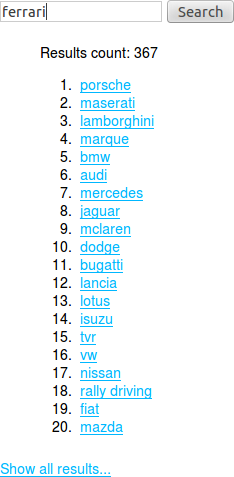
\includegraphics[height=0.6\textwidth]{figures/serelex}
        
\includegraphics[height=0.5\textwidth]{figures/spacer}
        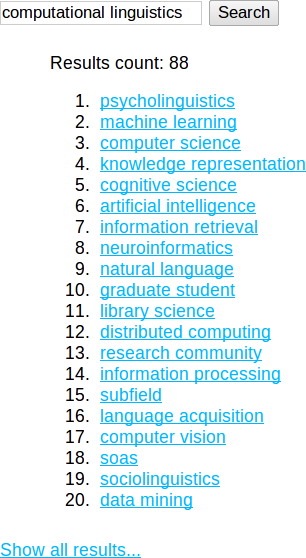
\includegraphics[height=0.6\textwidth]{figures/serelex-2}
        \end{figure}
\end{itemize}
\end{frame}







\begin{frame}
\frametitle{Lexico-syntactic patterns}

\begin{itemize}
  \item 18 patterns that extract \textbf{hypernyms}, \textbf{co-hyponyms} and \textbf{synonyms}
\begin{figure}  
    \centering
        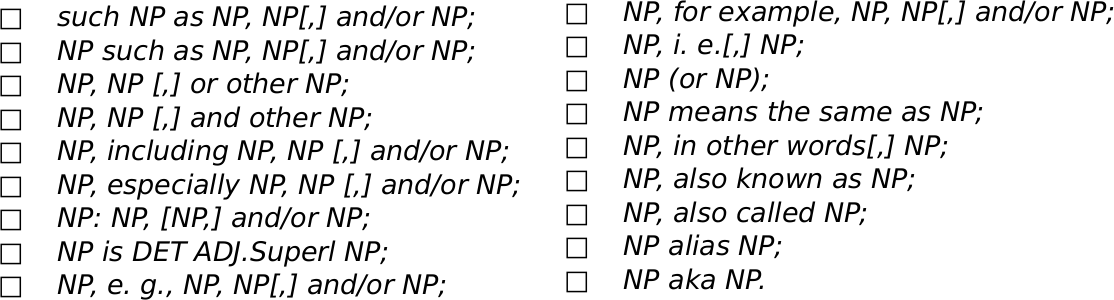
\includegraphics[width=1.0\textwidth]{figures/patterns}
    \end{figure}
\end{itemize}

\end{frame}




\begin{frame}
\frametitle{Patterns are encoded as FSTs}

\begin{itemize}
  \item Finite State Transducers (FSTs)
  \item Open source corpus processing tool \texttt{Unitex}: \url{http://igm.univ-mlv.fr/~unitex/}
  
\begin{figure}  
    \centering
        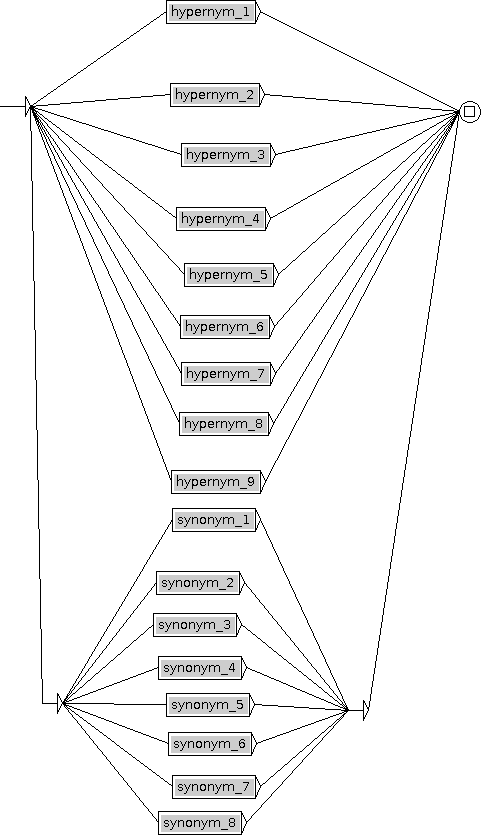
\includegraphics[width=0.3\textwidth]{figures/main-graph}
    \end{figure}
\end{itemize}

\end{frame}



\begin{frame}
\frametitle{A pattern encoded as an FST}

\begin{figure}  
    \centering
        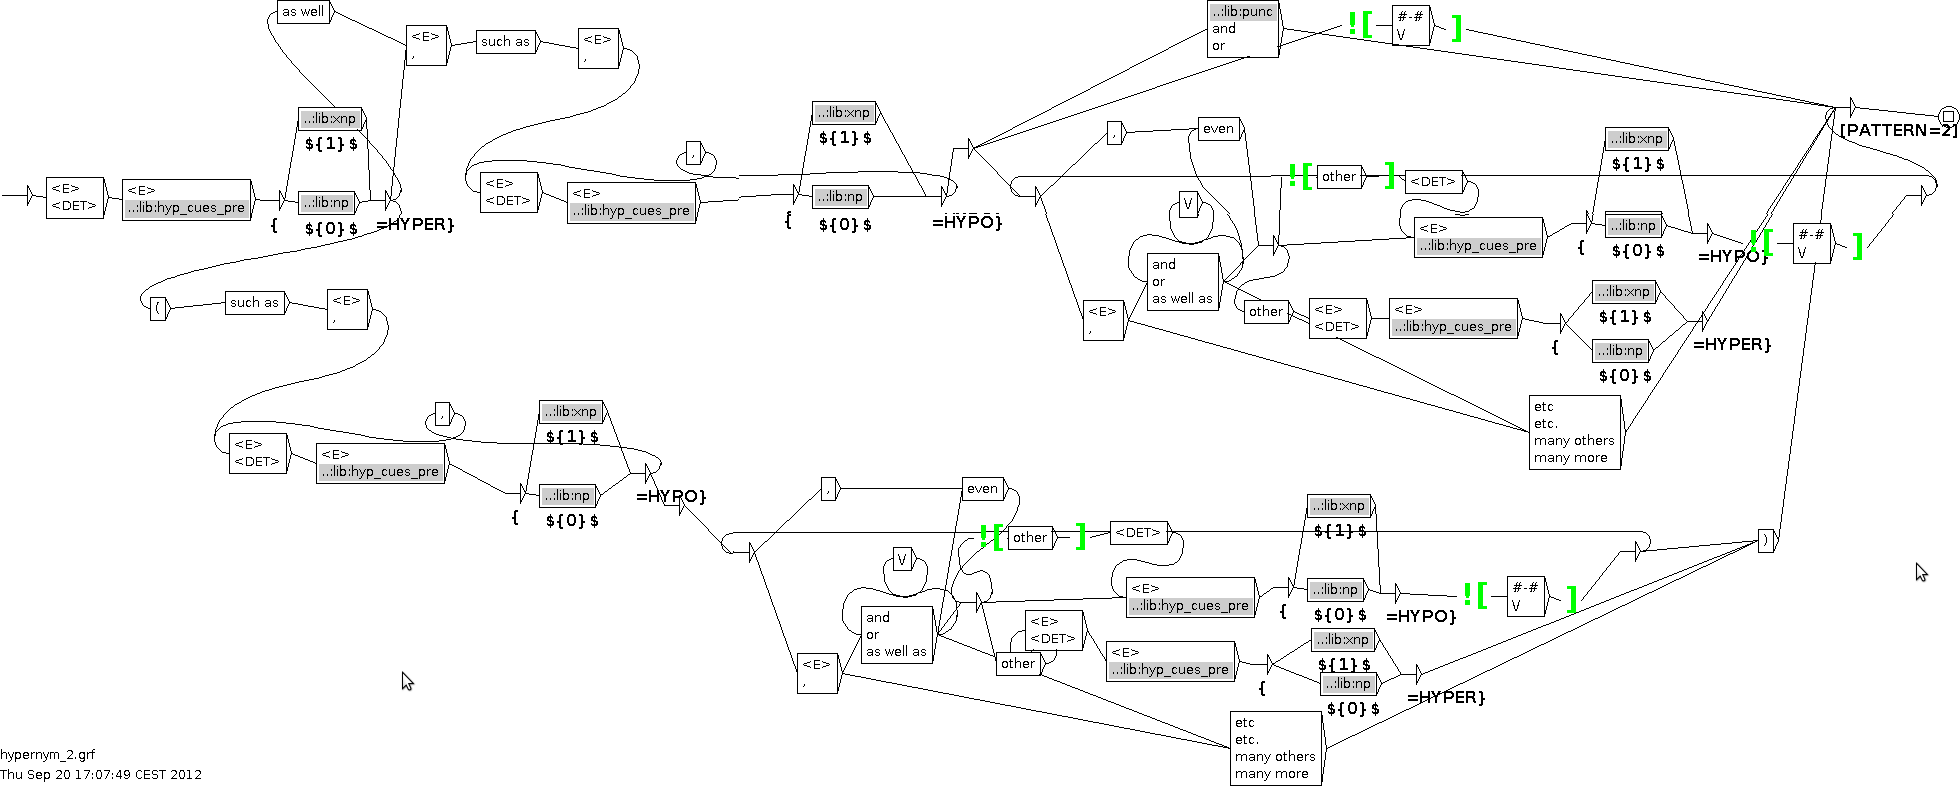
\includegraphics[width=1.0\textwidth]{figures/pattern2}
    \end{figure}

\begin{itemize}
  \item Take into account linguistic variation
  \item Unlike string-based patterns (Bollegala et al., 2007)
    
\end{itemize}

\end{frame}






\begin{frame}
\frametitle{Patterns extract concordances}

\begin{itemize}
  \item \texttt{such diverse \{[occupations]\} as
  \{[doctors]\}, \{[engineers]\} and \{[scientists]\}[PATTERN=1]}
  \item \texttt{such \{non-alcoholic [sodas]\} as \{[root beer]\} and \{[cream soda]\}[PATTERN=1]}
  \item \texttt{\{traditional[food]\}, such as \{[sandwich]\},\{[burger]\}, and \{[fry]\}[PATTERN=2]}
\end{itemize}

\end{frame}






\begin{frame}
\frametitle{Corpus}

\textbf{Corpus} Wikipedia+ukWaC: $2.9\cdot10^{12}$ tokens

\begin{figure}  
\centering
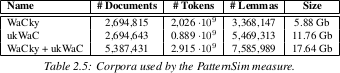
\includegraphics[width=0.7\textwidth]{figures/patternsim-table}
\end{figure}


\textbf{Extracted concordances}

\begin{itemize}
  \item Wikipedia -- 1.196.468 
  \item ukWaC -- 2.227.025 
  \item WaCypedia+ukWaC -- 3.423.493
\end{itemize}

\end{frame}





\begin{frame}
\frametitle{PatternSim Semantic Similarity}

  
$$s_{ij} = \sqrt{p_{ij}} \cdot \frac{2\cdot\mu_b }{b_{i*}+b_{*j}} \cdot \frac{P(c_i,c_j)}{P(c_i)P(c_j)}.$$


\begin{itemize}

%\item $s_{ij}$ -- semantic similarity between terms $c_i, c_j \in C$

\item $P(c_i,c_j)=\frac{e_{ij}}{\sum_{ij}e_{ij}}$ -- extraction probability of the pair $\langle c_i,c_j \rangle$, $e_{ij}$ --  frequency of co-occurrence of $c_i$ and $c_j$ in concordances $K$ 

\item $P(c_i)= \frac{f_i}{\sum_i f_i}$ -- probability of the term $c_i$, $f_i$ -- frequency of $c_i$ 
\item $b_{i*} = \sum_{j:e_{ij} \geq \beta} 1$ -- the number of extractions for term $c_i$ with the frequency $\geq \beta$, $\mu_b = \frac{1}{|C|}\sum_{i=1}^{|C|} b_{i*}$ -- the average number of extractions per term

\item $p_{ij} \in [1;18]$ -- number of distinct patterns which extracted the relation $\langle c_i, c_j \rangle$
  
 
\end{itemize}

\end{frame}




%\begin{frame}
%\frametitle{Semantic Relation Ranking}
%\begin{figure}	
%\centering
%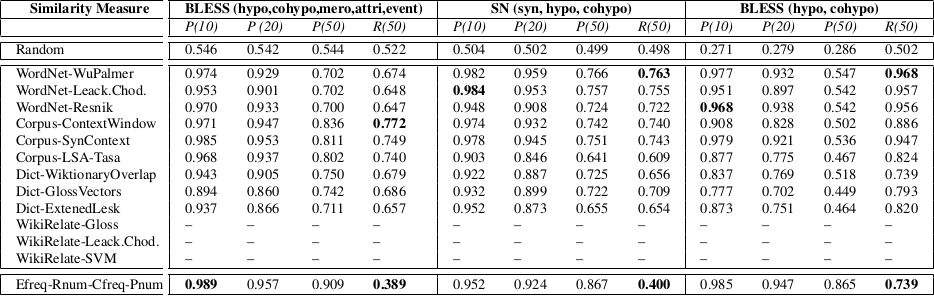
\includegraphics[width=1.0\textwidth]{figures/res-relations-mlg}
%\end{figure}
%\end{frame}




\begin{frame}
\frametitle{Semantic Relation Ranking}

\begin{itemize}
  \item Precision is \textbf{comparable or better} w.r.t. the baselines;
  \item Recall is \textbf{lower} w.r.t. the baselines.
\end{itemize}

\begin{figure}	
	\centering
	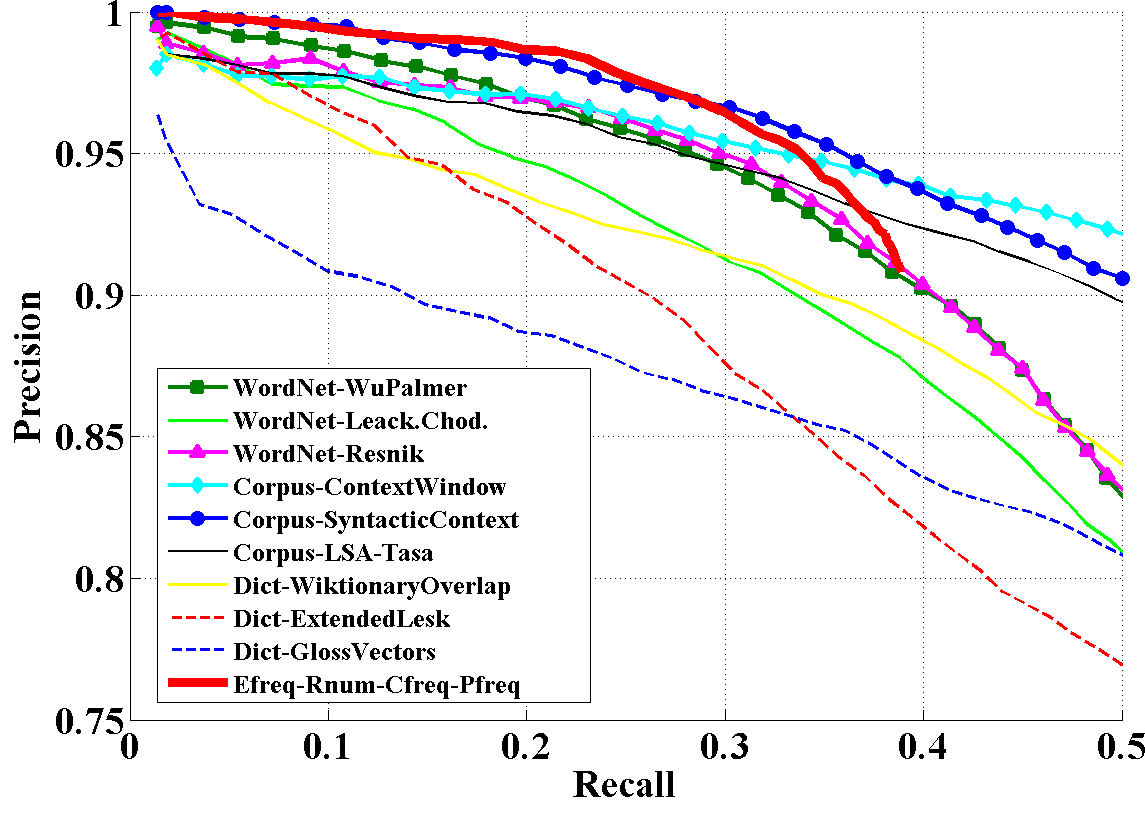
\includegraphics[width=0.65\textwidth]{figures/pr2-mlg}
	\caption{Precision-Recall graphs (the BLESS dataset).
	}
\end{figure}

\end{frame}





\begin{frame}
\frametitle{Semantic Relation Extraction}
  \begin{columns}[T]
    \begin{column}{.4\textwidth}
     
% Your text here
\includegraphics[width=0.85\textwidth]{./../figures/eval3}
    
    \end{column}
    \begin{column}{.6\textwidth}
    %\begin{block}{Your image}
\begin{itemize}
  %\item 49 words, three binary annotations;
  \item $Precision@1 \approx 0.80$;
  \item ``Good'' coverage:
  
\end{itemize}

\begin{figure}
\includegraphics[width=0.95\textwidth]{./../figures/wordnet-vs-serelex}
\end{figure}
      
    \end{column}
  \end{columns}
\end{frame}






%
%
%\section[Comparison]{Comparison of 
%Similarity Measures} 
%\subsection{  }
%
%
%
%
%\begin{frame}
%\frametitle{Related publications}
%
%\begin{itemize}
%
%\item Panchenko A. \textbf{A Study of Heterogeneous Similarity Measures for Semantic Relation Extraction.} // In JEP-TALN-RECITAL 2012 — Grenoble (France), 2012.
%
%\item Panchenko A., \textbf{Similarity Measures for Semantic Relation Extraction.} PhD thesis. Universit\'{e} catholique de Louvain. 197
%pages, 2013: \alert{Chapters 2.1, 3.1}. 
%
%\end{itemize}
% 
%\end{frame}
%
%
%
%
%\begin{frame}
%\frametitle{Compared Semantic Similarity Measures}
%
%\begin{figure}
%\includegraphics[width=1.0\textwidth]{./../figures/measures-classification}
%\end{figure}
%
%\begin{itemize}
%  \item 37 distinct measures;
%  \item \alert{Q1}: Are the measures are complementary?
%  \item \alert{Q2}: If yes, in which respects?
%\end{itemize}
% 
%\end{frame}
%
%
%
%
%
%
%
%
%
%\begin{frame}
%\frametitle{The Best Single Measures (MC, RG, WordSim, BLESS, SN)}
%
%\begin{figure}
%\includegraphics[width=1.07\textwidth]{./../figures/best}
%
%\end{figure}
%
%\begin{itemize}
%  \item Each one extracts many \alert{co-hyponyms}, e.g.: 
%  \begin{itemize}
%  \item $\langle Canon, Nikon \rangle$,
%  \item $\langle Lamborghini, Ferrari \rangle$,
%  \item $\langle Obama, Romney \rangle$.
%\end{itemize}
%\end{itemize}
%   
%\end{frame}
%
%
%
%\begin{frame}
%\frametitle{Further Results}
%
%\begin{columns}[T]
%
%\begin{column}{.6\textwidth}
%  
%\begin{block}{Most dissimilar measures}
%\begin{figure}
%\centering
%\includegraphics[width=1.0\textwidth]{./../figures/papers/7/figures/clusters-gray-2}   
%\caption{21 measures grouped according to their relation distributions. }
%\end{figure}
%\end{block}
%\end{column}
%
%\begin{column}{.4\textwidth}
%\begin{block}{Measures are  complementary w.r.t.:}
%\begin{itemize}
%  \item lexical coverage;
%  \item performances;
%  \item types of semantic relations they extract. 
%\end{itemize}
%\end{block}   
%\end{column}
%
%\end{columns}
%
%\end{frame}
%



%%%%%%%%%%%%%%%%%%%%%%%%%%%%%%%%%%%%%%%%%%%%%%%%%
\section[Hybrid Measures]{Hybrid Semantic Similarity Measure}

\subsection{}

\begin{frame}
\frametitle{Hybrid vs Single Measures}

\begin{figure}
\centering
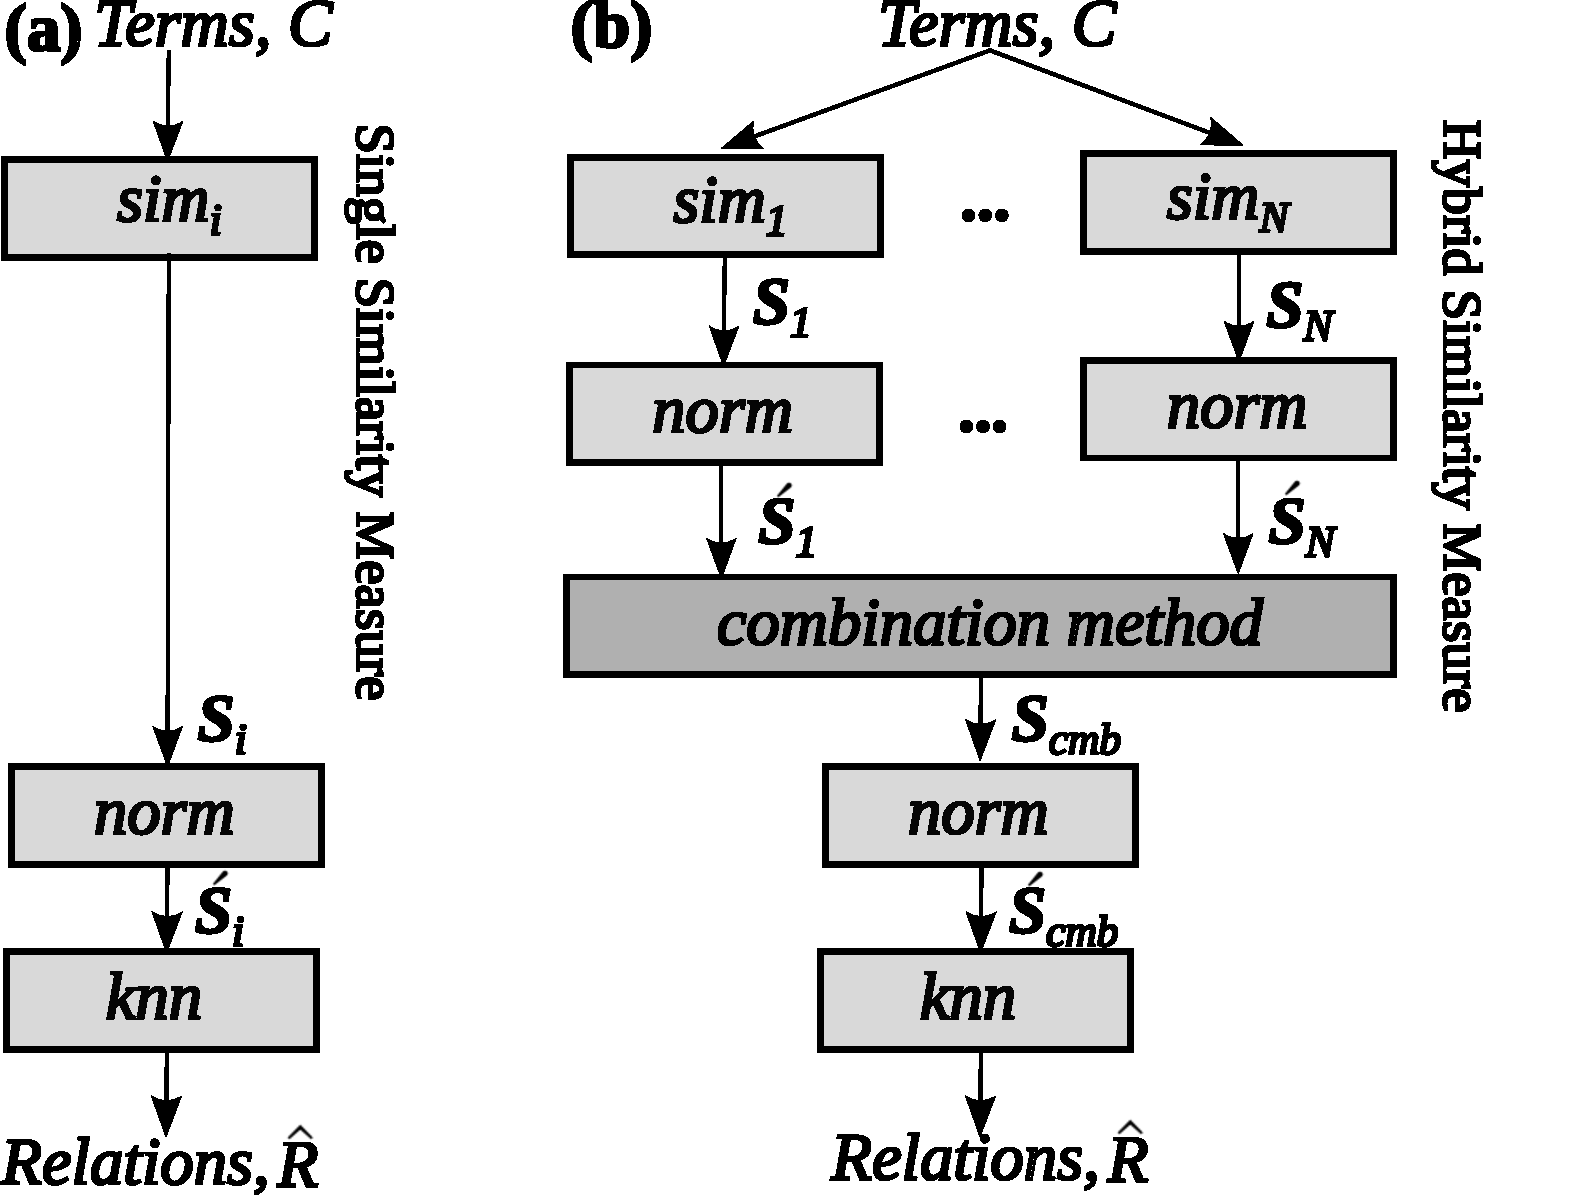
\includegraphics[width=0.65\textwidth]{./../figures/papers/4/src/figures/single-and-hybrid-2}
\caption{ Semantic relation extractor based on:
\begin{itemize}
\item \textbf{(a)} a \alert{single} similarity measure;
\item \textbf{(b)} a \alert{hybrid} similarity measure. 
\end{itemize}}
\end{figure}
\end{frame}





\begin{frame}
\frametitle{16 Features = 16 Single Similarity Measures}

	\begin{itemize}
	
	\item 5 \textbf{network-based} measures :
	\begin{enumerate}
	  \item WuPalmer;
	  \item Leacock and Chodorow;
	  \item Resnik;
	  \item Jiang and Conrath;
	  \item Lin.
	\end{enumerate} 
	\item 3 \textbf{web-based} measures (NGD-Yahoo/Bing/Google); 
		
	\item 5 \textbf{corpus-based} measures: 
	\begin{itemize}
	  \item 2 distributional (BDA, SDA)
	  \item 1 lexico-syntactic patterns (PatternSim)
	  \item 2 other co-occurence based (LSA, NGD-Factiva)
	\end{itemize}
	
	\item 3 \textbf{definition-based} measures
	\begin{enumerate}
	  \item ExtendedLesk;
	  \item GlossVectors;
	  \item DefVectors-WktWiki.
	\end{enumerate}
	 
\end{itemize}

\end{frame}




\begin{frame}
\frametitle{Implementation of the baseline measures}

\begin{itemize}
  \item \textbf{Semantic Vectors:} \url{https://code.google.com/p/semanticvectors/}
  \item \textbf{S-Space Package:} \url{https://code.google.com/p/airhead-research/}
  \item \textbf{WordNet::Similarity:} \url{http://wn-similarity.sourceforge.net}
  \item \textbf{NLTK:} \url{http://nltk.googlecode.com/svn/trunk/doc/howto/wordnet.html}
  \item \textbf{WikiRelate!}
  \item \textbf{PatternSim:} \url{http://serelex.org}
  \item \textbf{Web-based metrics:} \url{http://cwl-projects.cogsci.rpi.edu/msr}
  \item \textbf{LSA:} \url{http://lsa.colorado.edu}
  %\item \textbf{DefVectors:} \url{http://github.com/jgc128/defvectors}
\end{itemize}

\end{frame}






\begin{frame}
\frametitle{Supervised Combination of Measures}

\begin{enumerate}
  \setcounter{enumi}{7}
\item \textbf{Logistic Regression} 

\begin{itemize}
  \item  A binary \textbf{logistic regression};

\item \textbf{Positive examples} -- synonyms,
hyponyms, co-hyponyms;
\item \textbf{Negative examples} -- random relations;

  \item A relation $\langle c_i,t, c_j \rangle \in R$ is represented with a \textbf{vector of pairwise similarities}: $\mathbf{x} = (s_{ij}^1,\ldots,s_{ij}^N), N=\overline{2,16}$; 

\item Category $y_{ij}$:
$$
y_{ij} = \left\{ 
  \begin{array}{l l}
    0 & \quad  \text{ if } \langle c_i,t, c_j \rangle \text{ is a random relation} 
    \\
    1 & \quad  \text{ otherwise }\\
  \end{array} \right
  .
$$

\item \textbf{Using the model} $(w_1,\ldots,w_K)$ for combination: 
$$s^{cmb}_{ij} = \frac{1}{1 + e^{-z}}, z = \sum_{k=1}^K w_k s^k_{ij} + w_0.$$

\end{itemize}
\end{enumerate}

\end{frame}



\begin{frame}
\frametitle{Supervised Combination Methods}

\begin{enumerate}
  \setcounter{enumi}{8}
\item \textbf{SVM}. 


\begin{columns}
  \begin{column}{0.5\textwidth}
\begin{figure}
\centering
\includegraphics[width=1.0\textwidth]{./../figures/svm}
%\caption{SVM: maximal margin hyperplane. }
\end{figure}
    
  \end{column}

  \begin{column}{0.5\textwidth}
\begin{itemize}
\item The weights $\mathbf{w}$ and the support vectors $SV$: 

$$
\mathbf{w} = \sum_{x_i \in SV} \alpha_i y_i \mathbf{x}_i.  
$$

\item \textbf{Using the model} 

$$
s_{ij}^{cmb} = \mathbf{w}^T\mathbf{x} + b = \sum_{k=1}^K w_i s_{ij}^k + b.
$$

\end{itemize}    
  \end{column}
\end{columns}





\end{enumerate}

\end{frame}






\begin{frame}
\frametitle{Hybrid Similarity Measures}
\begin{figure}
\centering
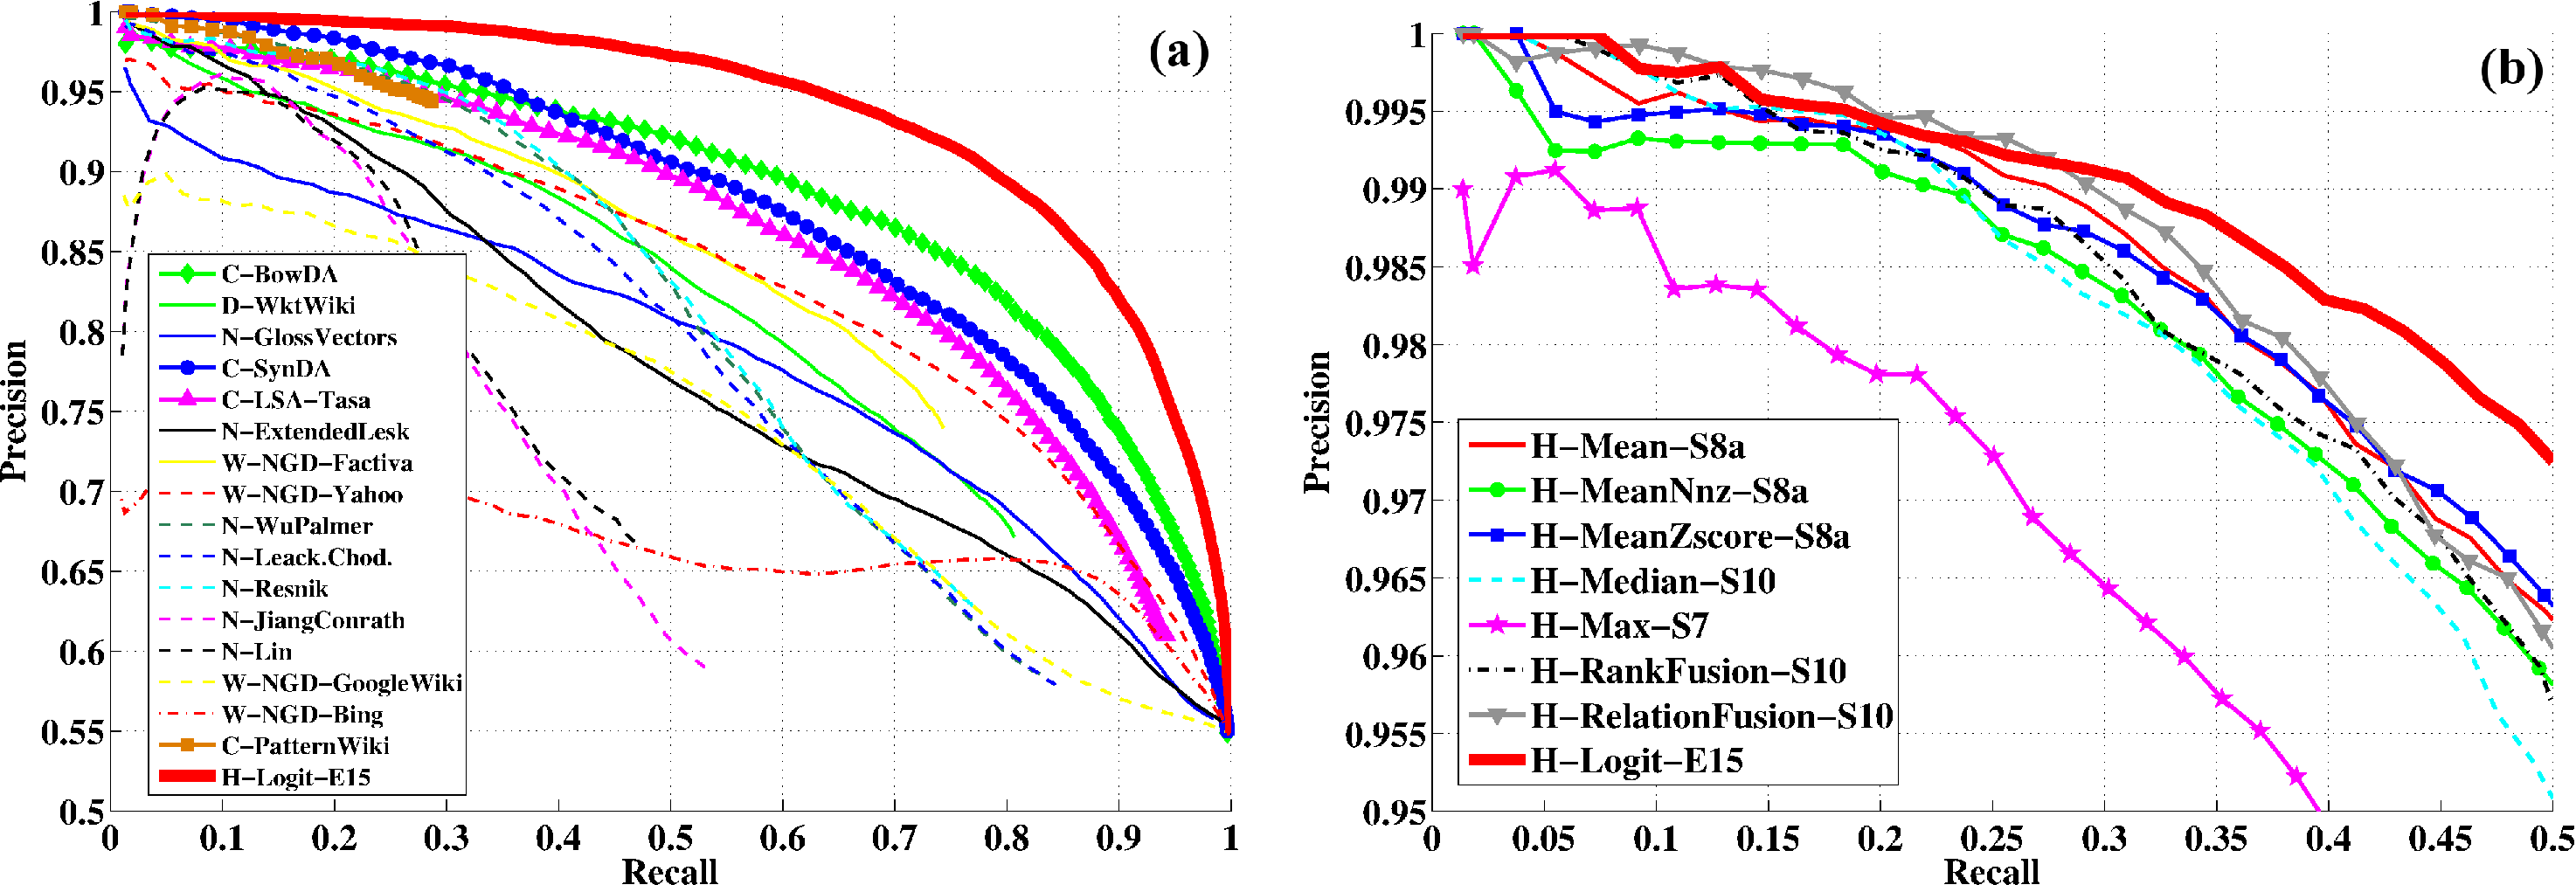
\includegraphics[width=1.0\textwidth]{figures/pr}
%\caption{

%}
\end{figure}

Precision-Recall graphs calculated on the BLESS dataset:
\begin{itemize}
  \item \textbf{(a)} 16 single measures and the best hybrid measure Logit-E15;
  \item \textbf{(b)} 8 hybrid measures.
\end{itemize}

\end{frame}



\begin{frame}
\frametitle{Supervised Hybrid Similarity Measures}
\begin{figure}
\centering
\includegraphics[height=0.4\textwidth]{./../figures/sn-accuracy}
\includegraphics[height=0.4\textwidth]{./../figures/bless-accuracy}
%
\includegraphics[height=0.025\textwidth]{./../figures/spacer}
%\includegraphics[height=0.36\textwidth]{./../figures/bless-precision10}
%\includegraphics[height=0.36\textwidth]{./../figures/bless-precision20}
%
\includegraphics[height=0.025\textwidth]{./../figures/spacer}
%\includegraphics[height=0.36\textwidth]{figures/bless-precision50}
%\includegraphics[height=0.36\textwidth]{figures/bless-recall50}     
     
\caption{ Meta-parameter optimization with the grid search of the C-SVM-radial-E15 measure.  }
\label{fig:radial-optimization}
\end{figure}
\end{frame}



\section[Word Embeddings]{Word Embeddings}

\begin{frame}
\frametitle{Key facts}

\textbf{Word embedding} is a dense vector representing a word obtained during a training of a neural network on a big corpus. 

\begin{itemize}
\item Semantic similarity is cosine of word embeddings. 

\item The training process is known as representation learning. 

\item Learning methods rely on distributional hypothesis of Harris (1954), similarly to classical distributional models. 

\item Most popular representation learning methods: 

\begin{itemize}
\item Continuous Bag of Words (CBOW) 

\item Skip-Gram Model 

\item Global Vectors of for Word Representation (GloVe)
\end{itemize}
\end{itemize}

\end{frame}



\begin{frame}
\frametitle{Distributional Hypothesis: "You shall know the word by the company it keeps" (Firth, 1957)}

\begin{figure}
\centering
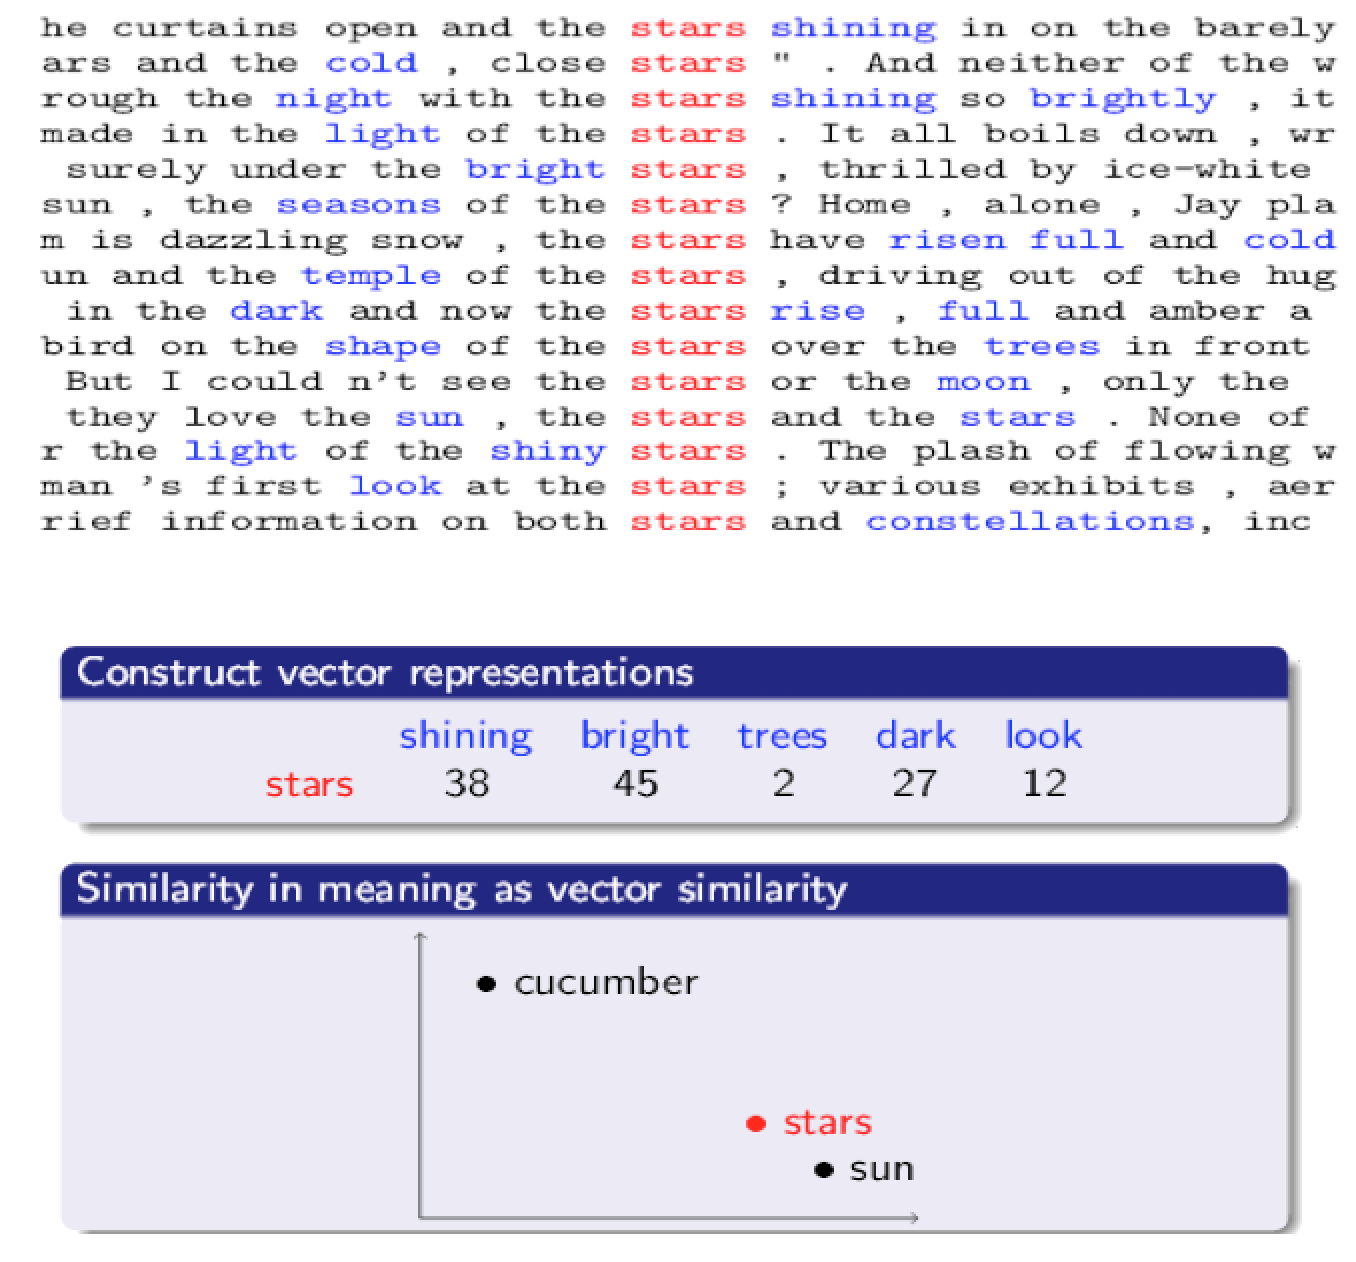
\includegraphics[height=0.91\textwidth]{./../grefenstette}
\end{figure}
	
\end{frame}




\begin{frame}

\frametitle{Skip-Gram Model}

\begin{itemize}

\item Probability that word $w$ appears in some context $c$:
{\small
$$ P(D=1| w,c;\theta) = \frac{1}{1+ \exp^{-V_c W_w}}$$  
}

\item Assign high probability to $(c,w$) pairs which appear in texts ($corp$) and low probability to the ones which cannot ($rand$): 
{\small 
$$\theta^* = arg max \prod_{(c,w) \in corp} P(D=1|w,c;\theta) \prod_{(c,w) \in rand} (1 - P(D=1|w,c;\theta))$$ 
}
\item $\theta = (V,W)$ are two matrices with columns $V_c$ and $W_w$ contain vectors of $dim$ dimensions of the context $c$ and the word $w$. 

\item The "embedding" of the word $w$ is the vector $W_w$. 


	
\end{itemize}

	
\end{frame}



\begin{frame}
\frametitle{Shared Task on Russian Semantic Similarity}

\begin{figure}  
    
\includegraphics[width=0.3\textwidth]{./../dialog_logo_en}
\end{figure}

\begin{itemize}
\item \url{www.dialog-21.ru/en/evaluation/2015/semantic}

\item  \textbf{Relatedness track}: Synonyms, Hypernyms, Human Judgements about Semantic Similarity
\item  \textbf{Associative track}: Free associations 
\end{itemize}

\end{frame}




\begin{frame}
\frametitle{ Evaluation }

\begin{figure}  
    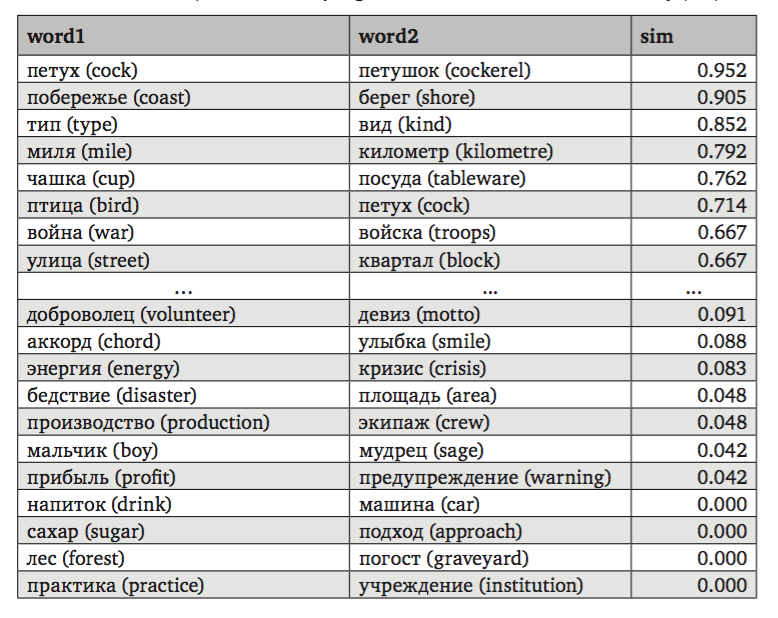
\includegraphics[width=0.8\textwidth]{../russe-evaluation}
\end{figure}

\end{frame}





\begin{frame}
\frametitle{ Best Systems }

\begin{figure}  
    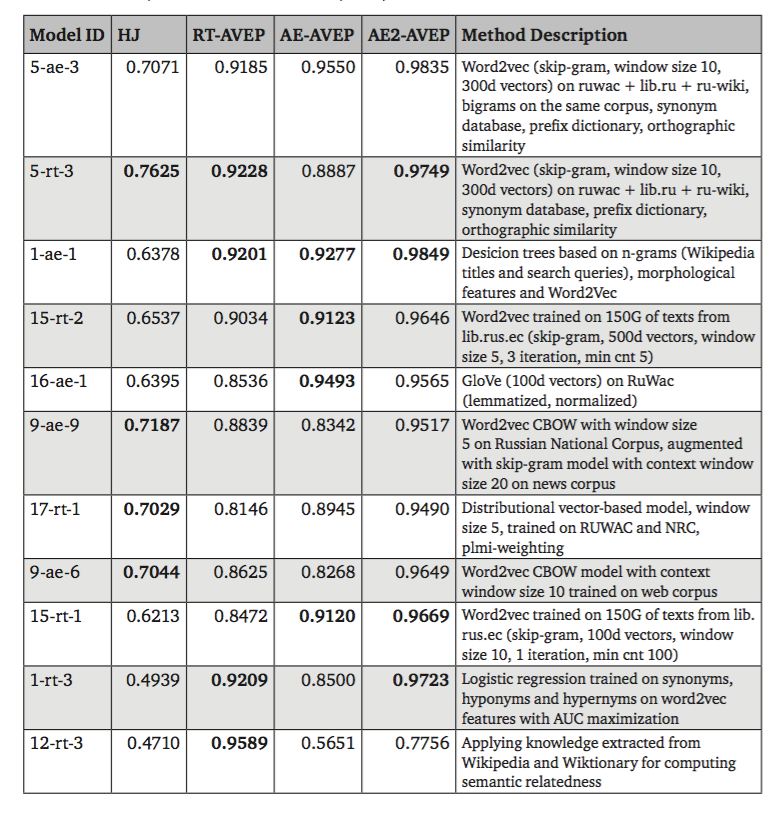
\includegraphics[width=0.65\textwidth]{../russe-results}
\end{figure}

\end{frame}


\begin{frame}
\frametitle{Skip-Gram on 150Gb of   lib.rus.ec corpus}
\begin{figure}
\centering
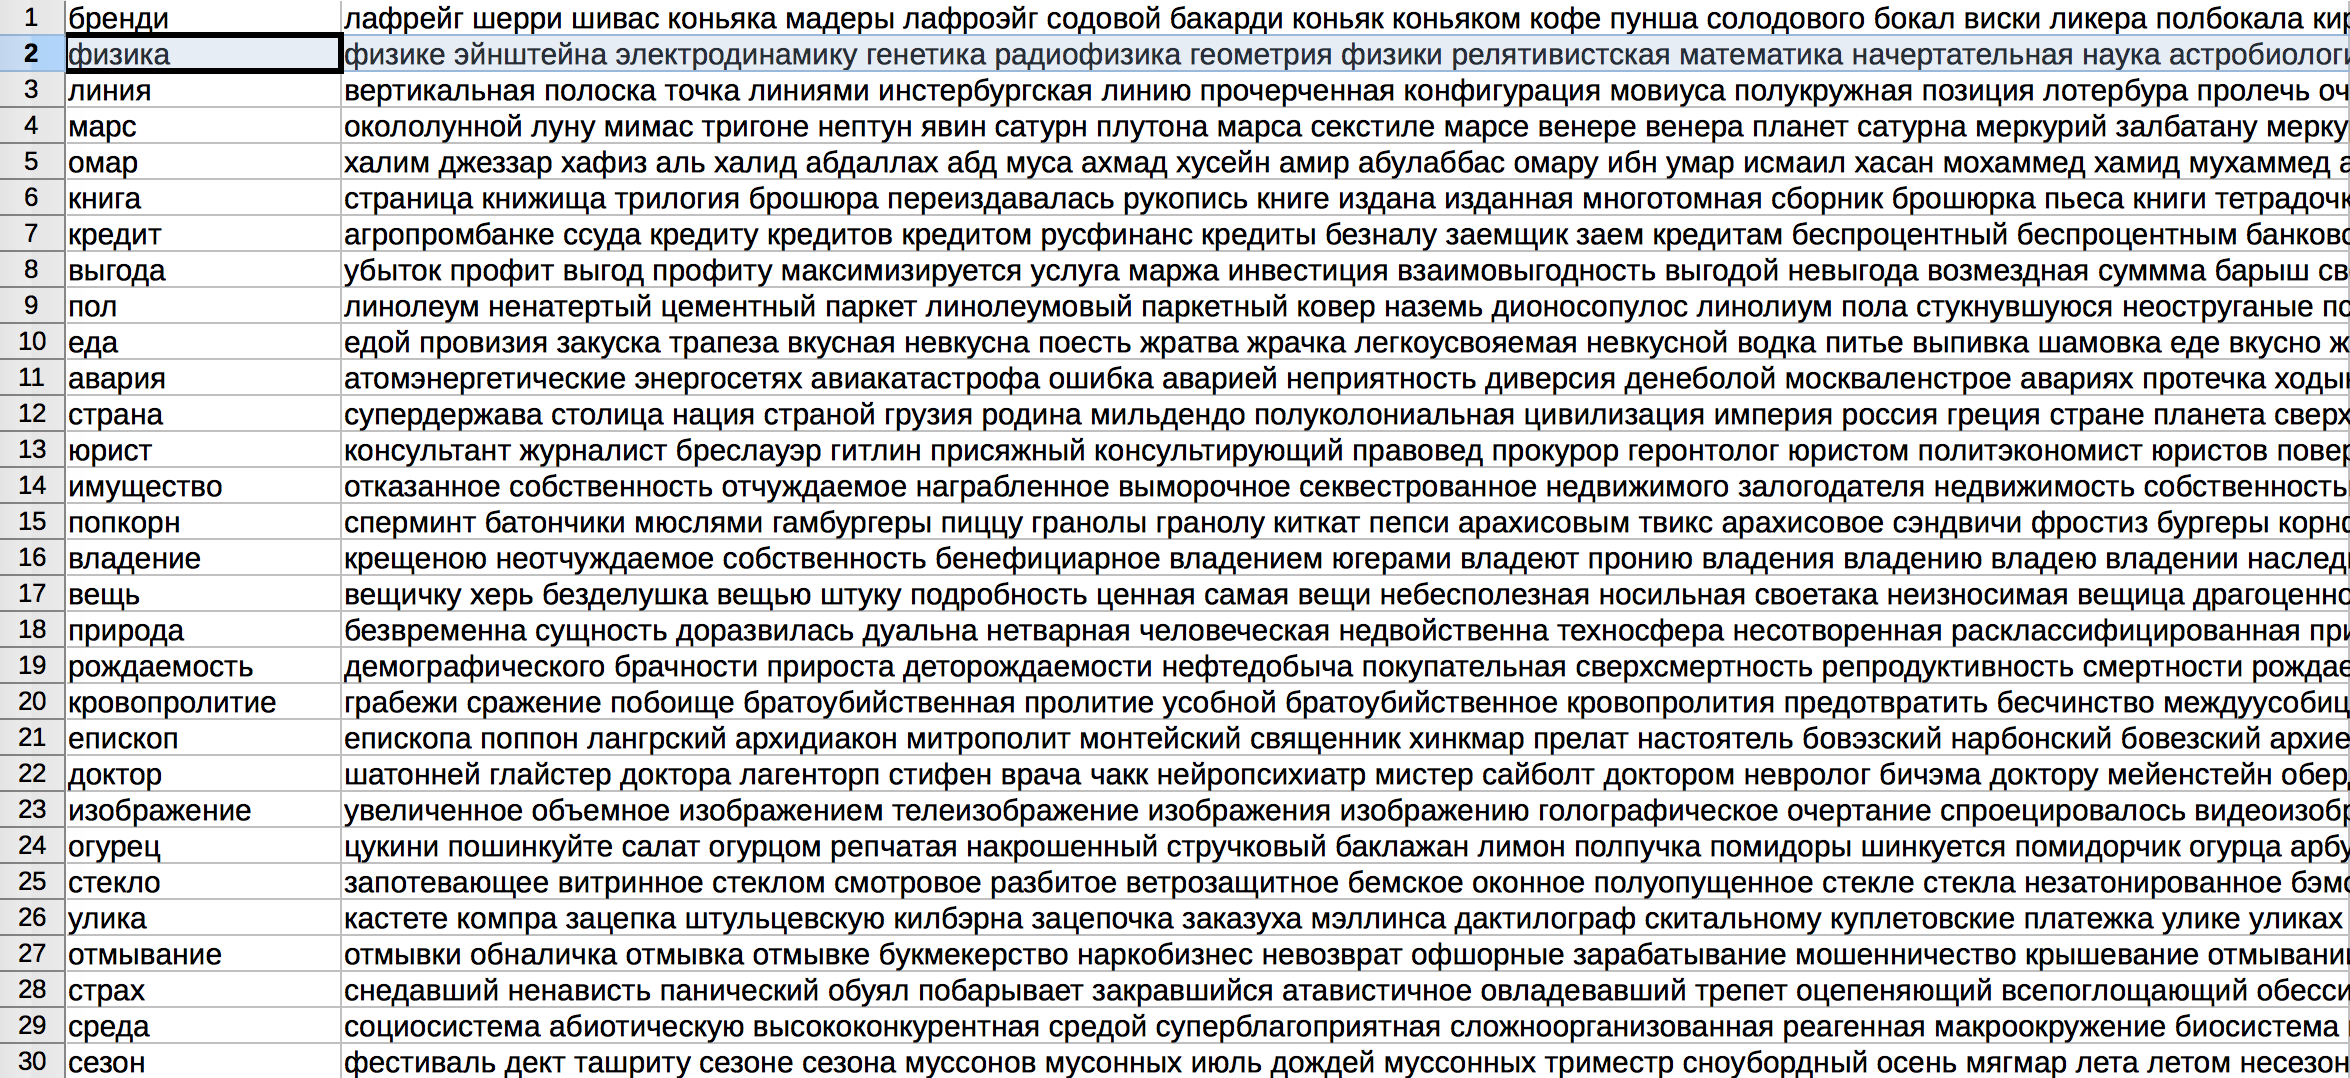
\includegraphics[width=1.0\textwidth]{./../dt-rus}
\end{figure}
	
\end{frame}



%
%
%\begin{frame}
%\frametitle{ Results: Semantic Relation Classification, Associations }
%
%\begin{figure}  
%    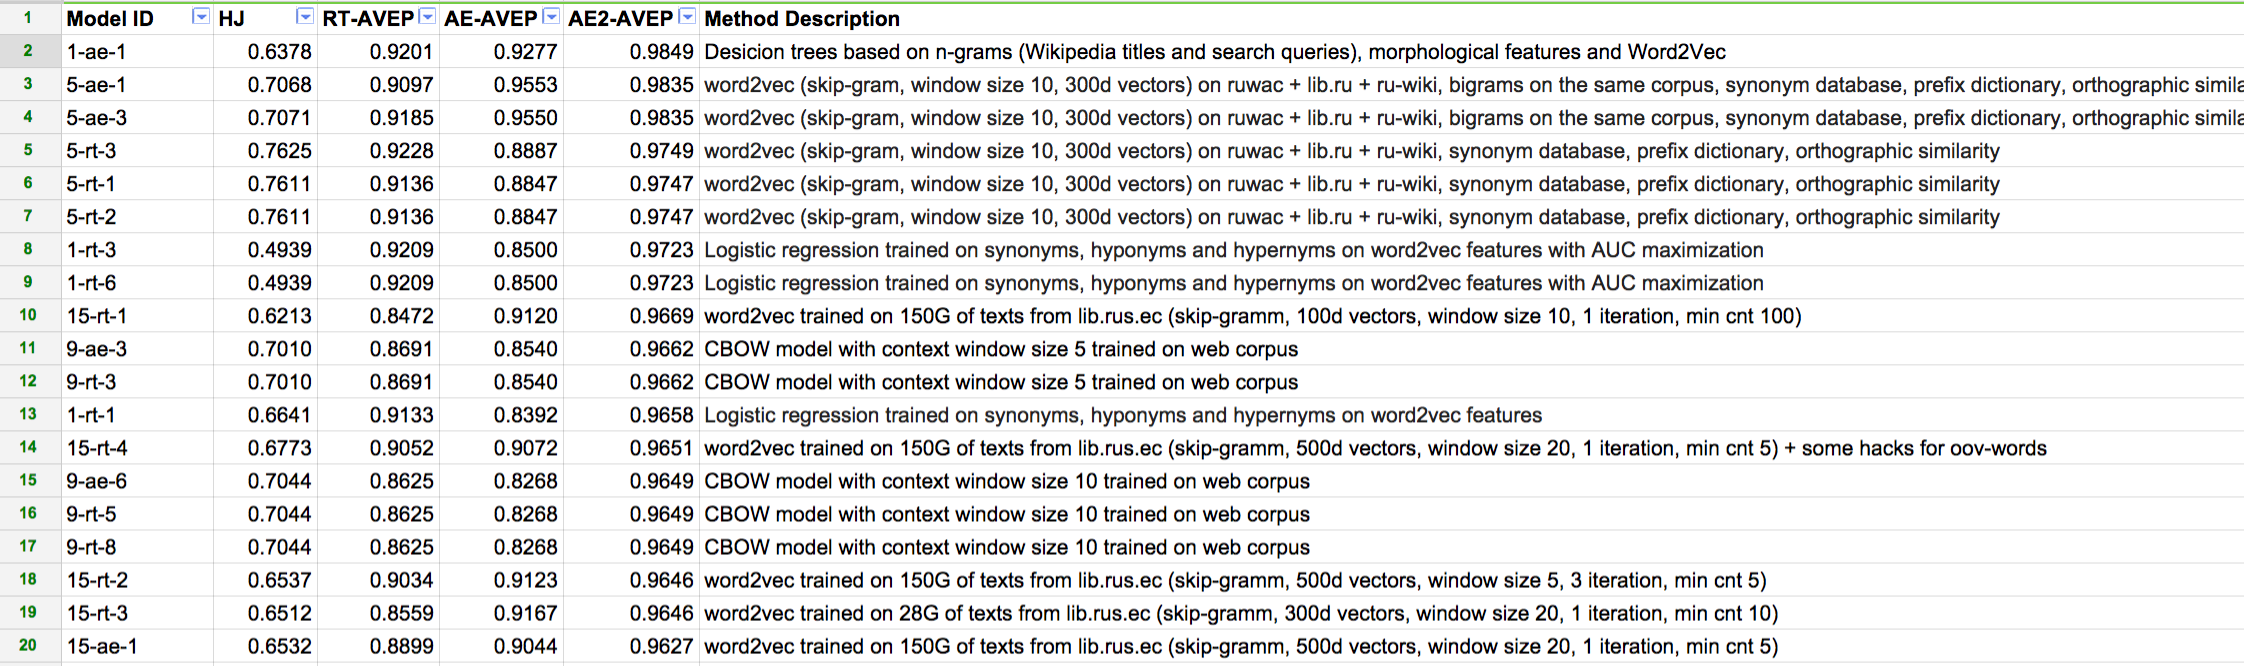
\includegraphics[width=1.45\textwidth]{figures/results-ae2}
%\end{figure}
%
%\end{frame}



%
\section[Lexical Semantics]{Computational Lexical Semanitcs}
\subsection{ }



\begin{frame}
\frametitle{Motivation}


\begin{figure}
\centering
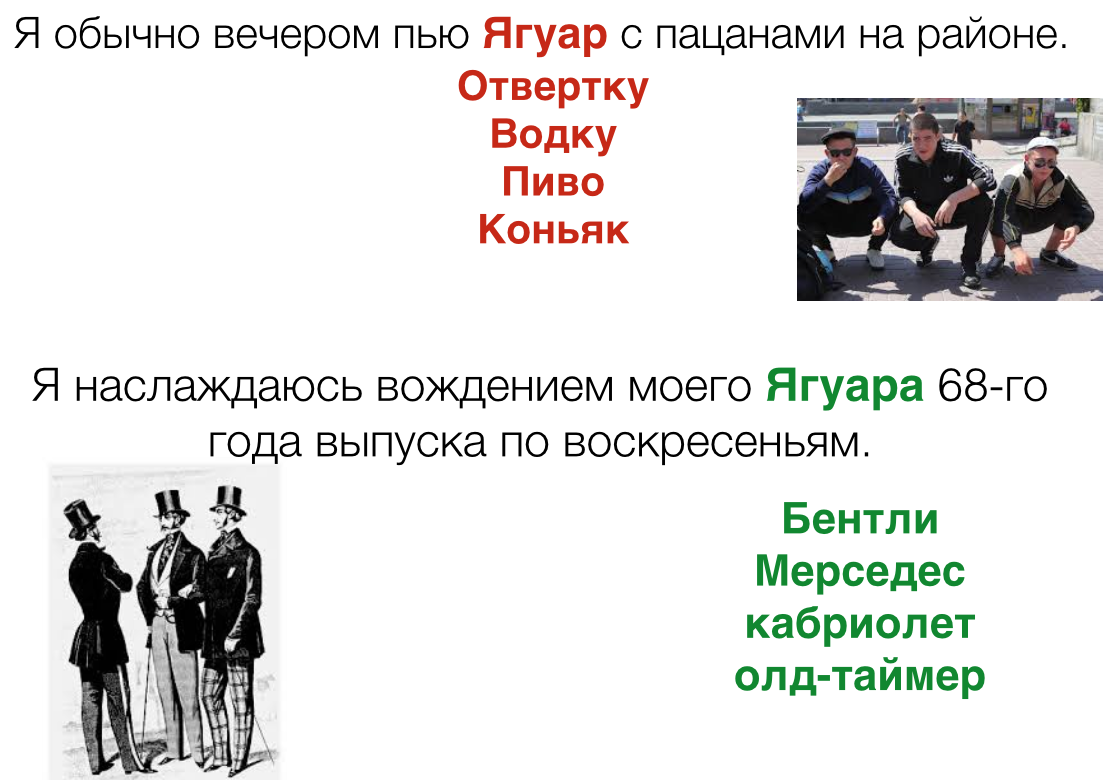
\includegraphics[width=0.95\textwidth]{./figures/jaguar}
\end{figure} 
\end{frame}


\begin{frame}
\frametitle{Two Worlds of Computational Lexical Semantics}


\begin{figure}
\centering
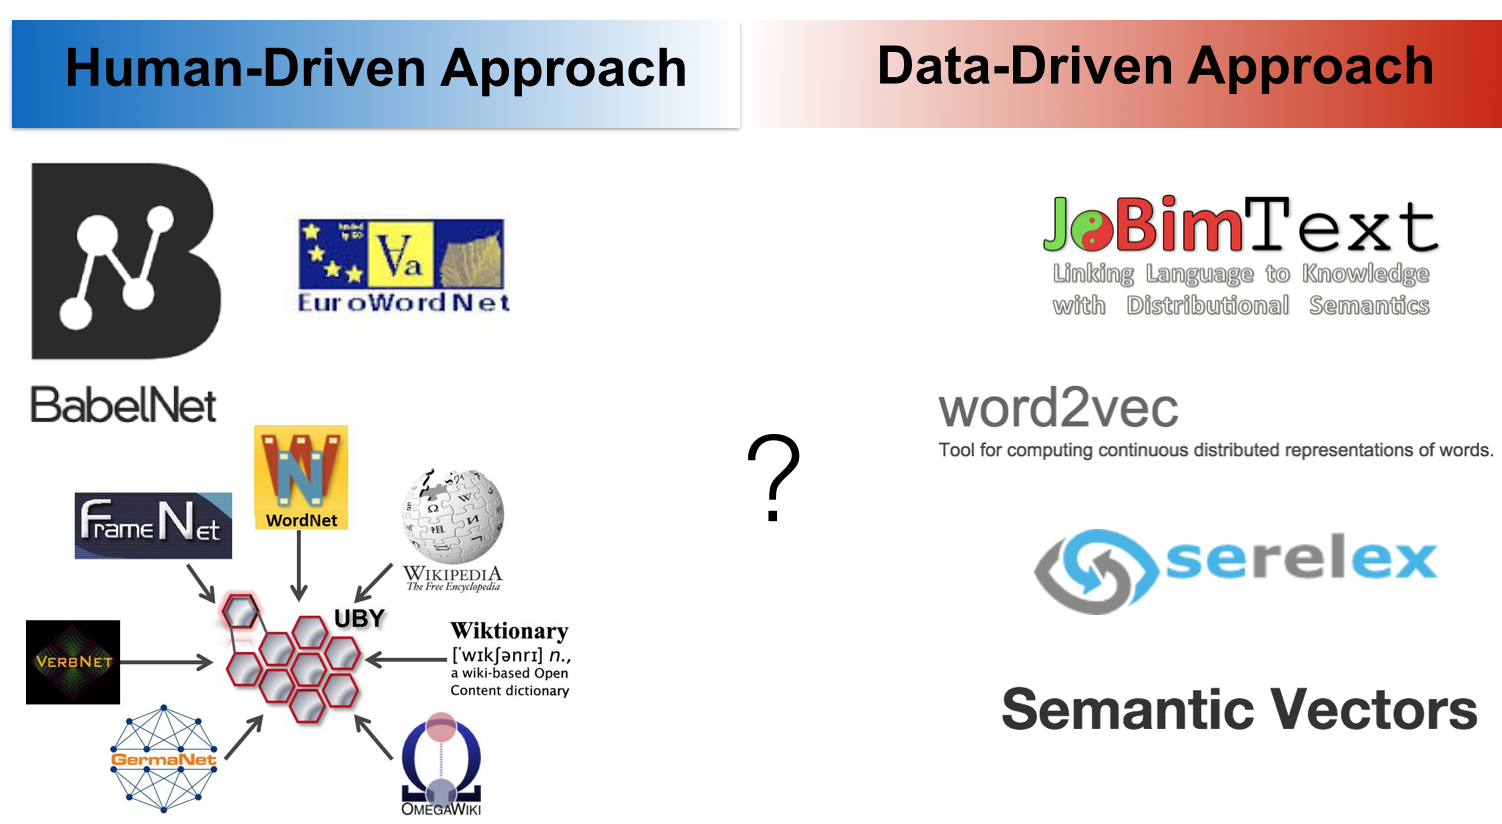
\includegraphics[width=1.0\textwidth]{./figures/two-worlds}
\end{figure} 
\end{frame}





\begin{frame}
\frametitle{Computational Lexical Semantics: Levels of Analysis}

\begin{figure}
\centering
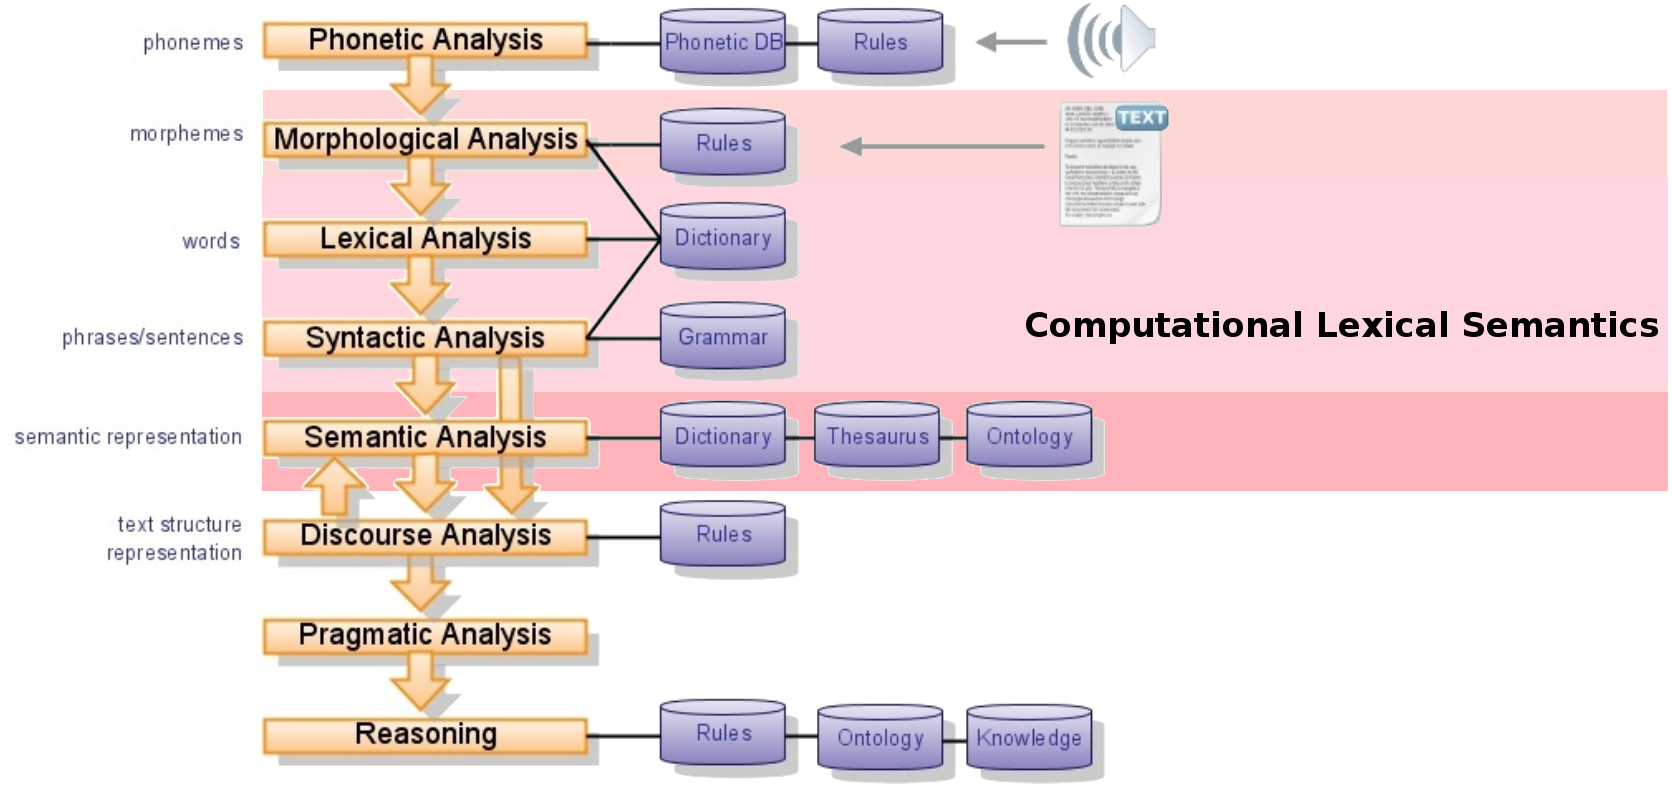
\includegraphics[width=1.05\textwidth]{figures/levels}
\end{figure}

 \tiny{* source of the image \url{http://www.uclouvain.be/en-cours-2013-LINGI2263.html}}

\end{frame}





\begin{frame}
\frametitle{Tasks}

\textbf{Computational models} of semantics of words and multiword expressions are used to solve following tasks:
 
\begin{itemize}
  \item Word sense disambiguation (WSD) and named entity disambiguation;
  \item Semantic relation extraction;
  \item Semantic similarity and semantic relatedness;
  \item Word sense induction (WSI) and discrimination;
  \item Generation of features for other NLP tasks.
\end{itemize}

\end{frame}




\begin{frame}
\frametitle{Introduction into the field}

\begin{itemize}
  \item Jurafsky D. and Martin J.H. An \textbf{Introduction to Natural Language Processing, Computational Linguistics, and Speech Recognition} (2009), chapters 19,20, 22.

\item Cruys T. \textbf{Mining for meaning: the extraction of lexico-semantic knowledge from text} (2010). PhD thesis. \url{http://dissertations.ub.rug.nl/faculties/arts/2010/t.van.de.cruys/} 

\item Panchenko A. \textbf{Similarity Measures for Semantic Relation Extraction} (2013) \url{http://cental.fltr.ucl.ac.be/team/~panchenko/thesis.pdf} 


\end{itemize}


\end{frame}



\begin{frame}
\frametitle{Key concepts}

\begin{itemize}
 \item \textbf{Lexical unit}: word, multiword expression (MWE), noun phrase (NP).
 \item \textbf{Vocabulary}: a set of words. 
 \item \textbf{Semantic relation}: defines a connection between lexical units. Relation can have a numerical weight and/or a type, such as synonymy, hypernymy, co-hyponymy or association. 
 \item \textbf{Semantic resource}: Vocabulary + a set of semantic relations. 
 \item \textbf{Distributional thesaurus}: a semantic resource without types. 
 \item \textbf{Semantic relatedness/similarity}: a numerical measure of word similarity.
 \item \textbf{Synset}: a group of mutual synonyms. 
 \item \textbf{Sense}: sense of a lexical item. 
 \item \textbf{Sense inventory:} a set of senses of a given vocabulary. 
\end{itemize}


\end{frame}



\begin{frame}
\frametitle{Semantic Resources}

\begin{block}{}

A \textbf{semantic resource} is an graph $(C, R)$:
\begin{itemize}
\item nodes $C$ represent \textbf{terms};
\item edges $R$ represent untyped \textbf{semantic relations}.
\end{itemize}

\end{block}

\begin{figure}
\centering
\includegraphics[height=0.400\textwidth]{./../figures/sr-29-example-crop2}
\end{figure}

\end{frame}




\begin{frame}
\frametitle{Semantic Relations}
\begin{figure}
\centering
\includegraphics[width=0.65\textwidth]{./../figures/sr-29-example}
\caption{A semantic resource composed of 29 relations.}
\end{figure}

\end{frame}





\begin{frame}
\frametitle{Types of semantic relaitons}

\begin{figure}
\centering
\includegraphics[height=0.49\textwidth]{./../figures/sr-example-2}
\includegraphics[height=0.35\textwidth]{./../figures/sr-example-spacer}
\includegraphics[height=0.43\textwidth]{./../figures/sr-example-untyped-2}
\caption{A semantic resource with (a) typed (b) untyped relations. }
\end{figure}

\end{frame}



\begin{frame}
\frametitle{Types of semantic relations}

\begin{figure}
\centering
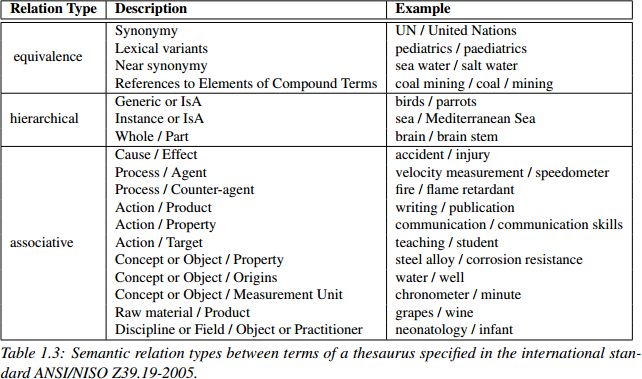
\includegraphics[height=0.49\textwidth]{./figures/sem-types}
\end{figure}

\end{frame}





\begin{frame}
\frametitle{Types of semantic relations}
\begin{figure}
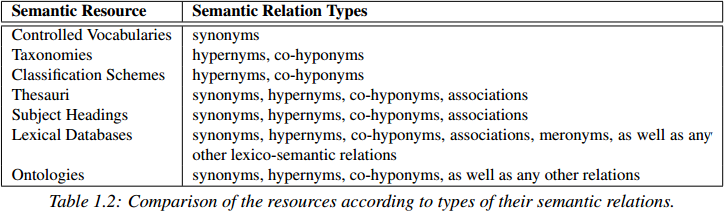
\includegraphics[width=1.0\textwidth]{figures/sem-res-table}
\end{figure}
\end{frame}







\frame{
\frametitle{Synsets}

\begin{figure}
\centering
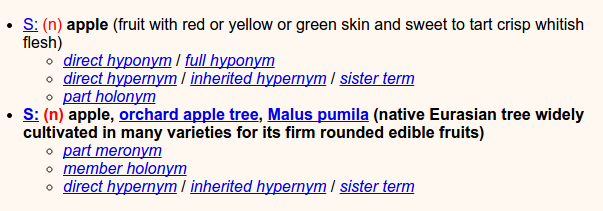
\includegraphics[width=0.9\textwidth]{figures/synset}
\caption{ WordNet synsets: \url{http://wordnetweb.princeton.edu/perl/webwn}. }
\end{figure}

}

\frame{
\frametitle{Synsets}

\begin{figure}
\centering
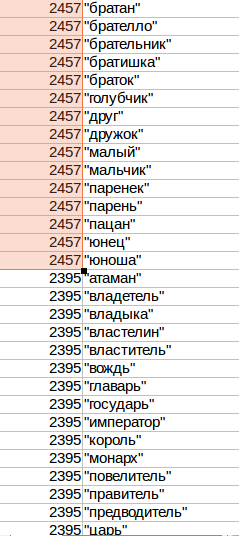
\includegraphics[width=0.26\textwidth]{figures/yarn}
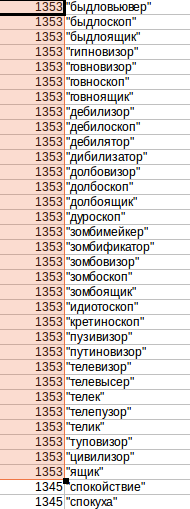
\includegraphics[width=0.22\textwidth]{figures/yarn2}
\caption{ YARN synsets: \url{http://russianword.net}. }
\end{figure}

}

\frame{
\frametitle{Synsets}

\begin{figure}
\centering
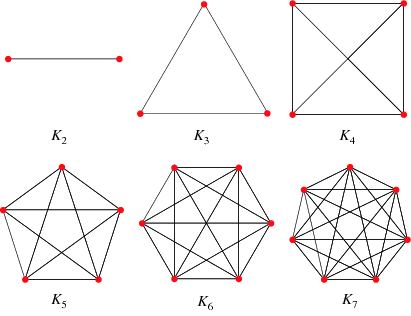
\includegraphics[width=0.7\textwidth]{figures/complete}
\caption{ Synset is a complete graph of synonyms. Source: \url{http://mathworld.wolfram.com/CompleteGraph.html}. }
\end{figure}

}

\begin{frame}
\frametitle{Semantic resources: expressiveness}

\begin{figure}
\centering
\includegraphics[width=0.9\textwidth]{../figures/expressivness}
\caption{ Expressiveness of different semantic resources. }
\label{fig:expressiveness}
\end{figure}

\end{frame}





\begin{frame}
\frametitle{Semantic resources: taxonomy }

\begin{figure}
\centering
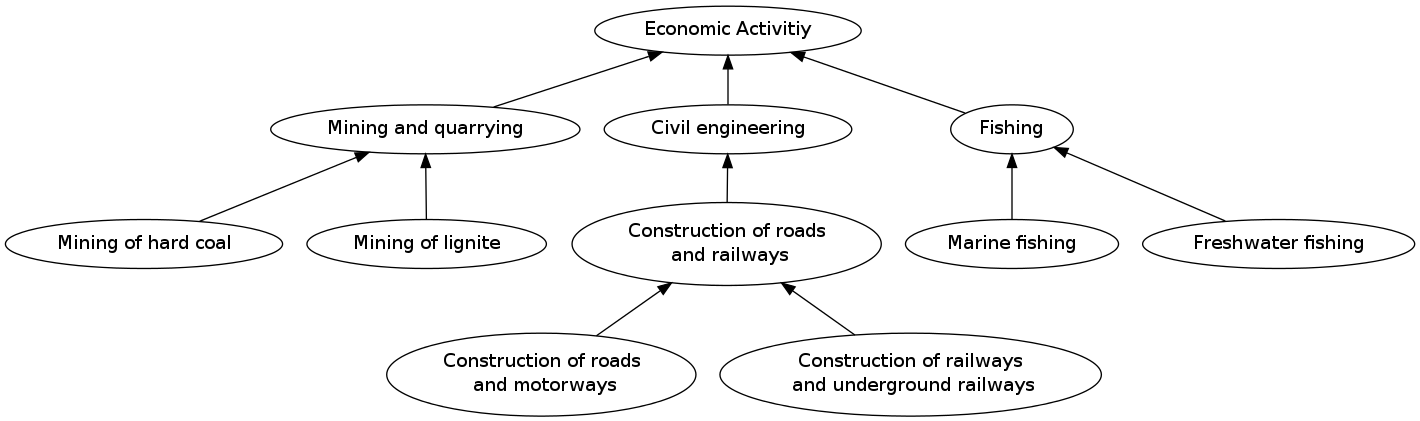
\includegraphics[width=1.0\textwidth]{figures/taxonomy-new}
\caption{ A part of the taxonomy of economical activities NACE.}
\label{fig:taxonomy}
\end{figure}

\end{frame}





\begin{frame}
\frametitle{Semantic resources: thesaurus }

\begin{figure}
\centering
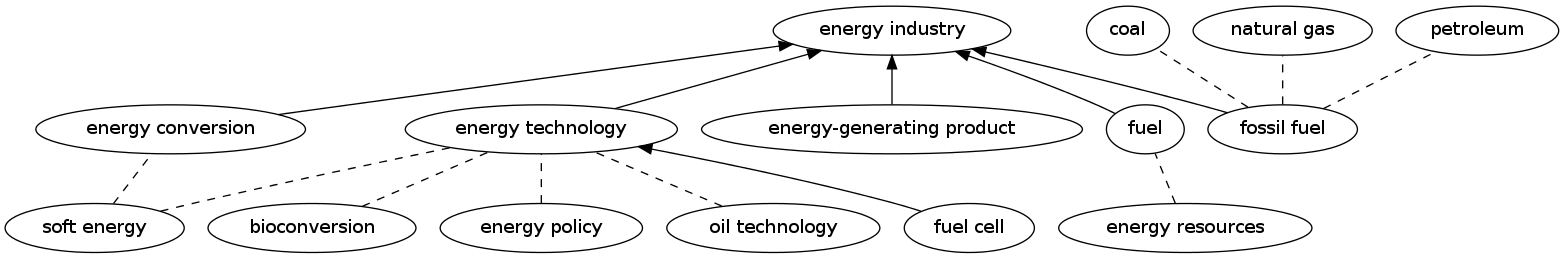
\includegraphics[width=1.0\textwidth]{figures/thesaurus-new}
\caption{ The Eurovoc thesaurus: the term ``energy industry'' and its semantic relations. Here, hypernyms are denoted with arrows and associations are denoted with dashed lines.}
\label{fig:thesaurus}
\end{figure}
\end{frame}




\begin{frame}
\frametitle{Semantic resources: lexical database }

\begin{figure}
\centering
\includegraphics[width=1.0\textwidth]{figures/wordnet-new}
\caption{ Lexical database WordNet: synset \textit{engineer} and its semantic relations. }
\label{fig:wordnet}
\end{figure}
\end{frame}


\begin{frame}
\frametitle{Semantic resources: lexical database}

\begin{figure}
\centering
\includegraphics[width=.7\textwidth]{figures/wnstat}
\caption{ WordNet statistics. Source: \url{https://wordnet.princeton.edu/wordnet/man/wnstats.7WN.html} }
\label{fig:wordnet}
\end{figure}
\end{frame}



\begin{frame}
\frametitle{Semantic Resources: WordNet}

\begin{figure}
\centering
\includegraphics[width=0.65\textwidth]{figures/wordnet-big}
\label{fig:wordnet}
\end{figure}

{\footnotesize \url{http://geniferology.blogspot.com/2012/10/playing-with-wordnet.html}}
\end{frame}





\begin{frame}
\frametitle{A multilingual WordNet: BabelNet.org}

\begin{figure}
\centering
\includegraphics[height=0.7\textwidth]{./figures/babelnet1}
\end{figure}

\end{frame}




\begin{frame}
\frametitle{A multilingual WordNet: BabelNet.org}

\begin{figure}
\centering
\includegraphics[height=0.7\textwidth]{./figures/babelnet2}
\end{figure}

\end{frame}





\begin{frame}
\frametitle{Semantic resources: ontology }

\begin{figure}
    \centering
        \includegraphics[width=1.0\textwidth]{../figures/ontology-new}
    \caption{ SUMO upper ontology: a part of the class hierarchy.}
    \label{fig:sumo}
\end{figure}
\end{frame}





\begin{frame}
\frametitle{Extraction of semantic resources from text }

\begin{figure}
\centering
\includegraphics[width=0.8\textwidth]{../figures/extraction-3}

\label{fig:semantic-relations-extraction}
\end{figure}

\end{frame}









\section[Semantic Similarity]{Semantic Similarity }
\subsection{ }




\frame{
\frametitle{Similarity Measures }

\begin{itemize}
  \item \textbf{Similarity measure} is a numerical measure of the degree the two objects are alike  
  \item \textbf{Dissimilarity measure} is a numerical measure of the degree to which the two objects are different.
  \item Both similarity and dissimilarity scores are scalars in range $[0;1]$ or $[0;\infty]$.
  \item Two similar objects $i$ and $j$ will have a high similarity score $s_{ij}$ and a low dissimilarity score $d_{ij}$.
  \item Similarity to dissimilarity and vice versa:
 \begin{itemize}
    \item if $d_{ij} \in [0;1]$, then $s_{ij} = 1 -d_{ij}$, where $s_{ij} \in [0;1]$;
    \item if $s_{ij} \in [0;1]$, then $d_{ij} = 1 - s_{ij}$, where $d_{ij} \in [0;1]$;
    \item if $d_{ij} \in [0;\infty]$, then $s_{ij} = 1 - \frac{d_{ij} - \min_{i,j}(d_{ij})}{\max_{i,j}(d_{ij}) - \min_{i,j}(d_{ij}) }$, where $s_{ij} \in [0;1]$;
    \item if $s_{ij} \in [0;\infty]$, then $d_{ij} = 1 - \frac{s_{ij} - \min_{i,j}(s_{ij})}{\max_{i,j}(s_{ij}) - \min_{i,j}(s_{ij}) }$, where $d_{ij} \in [0;1]$.
\end{itemize}
\end{itemize} 

\textit{Definitions are adapted from (Tan, 2006).}


}



\begin{frame}
\frametitle{Semantic Similarity Measures}



\begin{block}{Definition}
  A semantic similarity measure quantifies semantic relatedness input terms $c_i, c_j$ with the similarity score $s_{ij} = sim(c_i,c_j)$:
    $$
  s_{ij} = \left\{ 
   \begin{array}{l l}
     1 & \quad \text{if } \langle c_i, c_j \rangle \text{ is a pair of } syn, hyper, cohypo \\
    0 & \quad \text{otherwise}\\
   \end{array} \right.
 $$
 \end{block}


\begin{block}{Properties}
\begin{itemize}    
  \item Nonnegativity: $0 \leq s_{ij} \leq 1$;
  \item Reflexivity: $s_{ij} = 1 \Leftrightarrow c_i = c_j$;
  \item Symmetricity: $s_{ij} = s_{ji}$;
  \end{itemize}
 \end{block}
     
\end{frame}



\frame{
\frametitle{Word similarity matrix $\mathbf{S}$}


\begin{itemize}
\item  $\mathbf{S}$ -- word $*$ word similarity matrix;
\item $s_{ij} \in \mathbf{S}$ -- similarity of words $w_i$ and $w_j$;
\item $s_{ij} = sim(w_i, w_j), s_{ij} \in [0;1].$
\end{itemize}

\begin{figure}
\centering
\includegraphics[width=0.5\textwidth]{./figures/simm}
\end{figure}

}




\begin{frame}
\frametitle{Semantic Similarity Measures}
\begin{itemize}

\item Many dissimilar pairs, few similar pairs: $s_{ij} \sim exp(\lambda)$:

\begin{figure}
\centering
\includegraphics[width=0.5\textwidth]{./../figures/reldist-crop}
\end{figure}

\item Similarity distribution of the term ``doctor'': 

\begin{figure}
\centering
\includegraphics[width=0.6\textwidth]{./../figures/real-extracted}
\end{figure} 

\end{itemize}
\end{frame}




\begin{frame}
\frametitle{Number of relations in semantic resources}
\begin{figure}
\centering
\includegraphics[width=0.9\textwidth]{./../figures/reldist}
\caption{ Number of relations (synonyms and hyponyms) per term in the dictionaries: a dictionary of synonyms, Roget's thesaurus, WordNet and a union of these three resources.  }
\label{fig:sim-distribution}
\end{figure}

\end{frame}


\begin{frame}
\frametitle{Evaluation of Semantic Similarity Measures}

\begin{enumerate}
\item correlations with human judgments (\textbf{MC}, \textbf{RG}, \textbf{WordSim});
\item semantic relation ranking (\textbf{BLESS}, \textbf{SN});
\item semantic relation extraction;
\item using extracted relations in an application:
\begin{itemize}
\item a short text classification system (\textbf{iCOP});
\item a lexico-semantic search engine (\textbf{Serelex}).
\end{itemize}
\end{enumerate}

\end{frame}









\begin{frame}
\frametitle{Evaluation of Semantic Similarity Measures}

\begin{enumerate}
\item \textbf{Correlations with human judgments}:
\begin{itemize}
 \item Criterion: Pearson correlation ($\rho$) О Spearman correlation ($r$).
 \item Datasets: MC, RG, WordSim.
\end{itemize}

\item \textbf{Semantic relation ranking}:
\begin{itemize}
 \item Criterion: Precision, Recall, F-measure.
 \item Dataset: BLESS, SN.
\end{itemize}


\item \textbf{Semantic relation extraction:}
\begin{itemize}
 \item Criterion: Precision@k.
 \item Data: annotation and/or dictionaries.
\end{itemize}

\item \textbf{Application-based evaluation:}
\begin{itemize}
\item short text classification system (\textbf{iCOP});
\item lexico-semantic search engine (\textbf{Serelex}).
\end{itemize}
\end{enumerate}


Panchenko A., \textbf{Similarity Measures for Semantic Relation Extraction.} PhD thesis. Universit\'{e} catholique de Louvain. 197 pages, 2013, (Chapter 1). 

\end{frame}







\begin{frame}
\frametitle{Correlations with human judgments}

\begin{table}[h]\footnotesize
\begin{tabular}{ |c|c|c|c|c|c| }
\hline
  word, $c_i$ & word, $c_j$ & human, $\mathbf{s}$  & sim, $\mathbf{s}$  & human (rank), $\mathbf{r}$ & sim (rank), $\hat{\mathbf{r}}$  \\ \hline \hline
tiger & cat & 7.35 & 0.85 & 1 & 3 \\
book & paper & 7.46 &  0.95 & 2 & 2 \\
computer & keyboard & 7.62 &  0.81 & 3 & 1 \\
... & ... & ... & ...   & \ldots & \ldots \\
possibility & girl & 1.94 & 0.25 & 64 & 65 \\
sugar & approach & 0.88 & 0.05 & 65 & 23 \\ \hline
\end{tabular}
\end{table}


\textbf{Datasets:}

\begin{itemize}
    \item WordSim353 -- 353 word pairs (Finkelstein, 2002)  
    \item MC -- 30 word pairs  (Miller & Charles, 1991)
    \item RG -- 65 word pairs (Rubenstein & Goodenough, 1965)  
\end{itemize}

\textbf{Pearson correlation:}  $\rho = \frac{cov(\mathbf{s},\hat{\mathbf{s}})}{\sigma(\mathbf{s}) \sigma(\hat{\mathbf{s}})}$

 \textbf{Spierman correlation:}: $r = \frac{cov(\mathbf{r},\hat{\mathbf{r}})}{\sigma(\mathbf{r}) \sigma(\hat{\mathbf{r}})}$
\end{frame}



\begin{frame}
\frametitle{Correlations with human judgments}

\begin{figure}
\includegraphics[height=0.6\textwidth]{./figures/rg}
\end{figure}


\end{frame}



\begin{frame}
\frametitle{Correlations with human judgments}

\begin{figure}
    \centering
        \includegraphics[width=0.55\textwidth]{../figures/mc-correlations-2}
    \caption{ Spearman correlation on the Miller-Charles (MC) dataset. $\rho$ of a similarity measure is 0.843 (p<0.001) and $\rho$ of a random measure is -0.173 (p=0.360). }
    \label{fig:mc-correlations}
\end{figure}
\end{frame}



%%%%%%%%%%%%%%%%%%%%%%%%%%%%%%%%%%%%%%%%%%%%%%%%%



%%%%%%%%%%%%%%%%%%%%%%%%%%%%%%%%%%%%%%%%%%%%%%%%%
\begin{frame}
\frametitle{Semantic Relation Ranking and Classification}

{ \scriptsize

\begin{table}[h]\footnotesize
\begin{tabular}{ |c|l|l| }
\hline
\bf слово, $c_i$ & \bf  слово, $c_j$ & \bf тип отношения, $t$  \\ \hline \hline
judge & adjudicate & syn \\
judge & arbitrate & syn \\
judge & asessor & syn \\
... & ... & ...   \\
judge & pc & random \\ 
judge & fare & random \\
judge & lemon & random \\ \hline
\end{tabular}
\end {table}

}

\textbf{Datasets:}
\begin{itemize}
  \item BLESS (Baroni and Lenci, 2011)  -- 26554 relations (hyper, coord, mero, event, attri, random)  
  \item SN (Panchenko, 2012) -- 14682  relations (syn, random) 
 \item RT, AE, AE2 (Panchenko et al., 2015)

\end{itemize}

\end{frame}



\begin{frame}
\frametitle{Semantic Relation Ranking  and Classification}

\begin{itemize}
   \item Precision $P(k=50)= \frac{1}{7} \approx 0.86 $
\end{itemize}


\begin{table}[h]\footnotesize
\begin{tabular}{ |l|l|l|l| }
\hline
\bf word, $c_i$ & \bf  word, $c_j$ & \bf relation type & \bf $s_{ij}$ \\ \hline \hline

aficionado & enthusiast & syn & 0.07197 \\
aficionado & fan & syn & 0.05195 \\
aficionado & admirer & syn & 0.01964 \\
aficionado & addict & syn & 0.01326 \\
aficionado & devotee & syn & 0.01163 \\
\alert{aficionado} & \alert{foundling} & \alert{random} & \alert{0.00777} \\
aficionado & fanatic & syn & 0.00414 \\ \hline
aficionado & adherent & syn & 0.00353 \\
aficionado & capital & random & 0.00232 \\
aficionado & statute & random & 0.00029 \\
aficionado & blot & random & 0.00025 \\
aficionado & meddler & random & 0.00005 \\
aficionado & enlargement & random & 0.00003 \\
aficionado & bawdyhouse & random &  0.00000 \\ 
\hline
\end{tabular}
\end {table}

\end{frame}



\begin{frame}
\frametitle{Semantic Relation Ranking  and Classification: BLESS}

\begin{table*}
\centering
%\caption{A target word ``hawk" and all its relatum words from the BLESS dataset ranked by similarity score. The table on the left      contains relations retrieved with the $k$-NN threshold of 50$\%$ The whole table contains all relations of the word ($k=100\%). }
\includegraphics[width=0.55\textwidth]{../figures/bless-example}
\label{tbl:bless-example}
\end{table*}
    
\end{frame}


%%%%%%%%%%%%%%%%%%%%%%%%%%%%%%%%%%%%%%%%%%%%%%%%%
\begin{frame}
\frametitle{Semantic Relation Ranking  and Classification}

\begin{itemize}
  
  \item Based on the number of  \alert{correctly classified or ranked} semantic relations.
  

\item $R$ -- set of non-random relations, e.g. not like $\langle animal, random, bishop \rangle$

\item $\hat{R}(k)$ set of extracted relations at $k$ nearest neighbours

\begin{block}{Evaluation metrics}

    
    \begin{itemize}
        \item Precision: $P(k)=$$\frac{|R \cap \hat{R}(k)|}{|\hat{R}(k)|}$,
        \item Recall: $R(k)=$$\frac{|R \cap \hat{R}(k)|}{|R|}$,
        \item F1-measure: $F(k)= 2 \cdot \frac{P(k) \cdot R(k)}{P(k) + R(k)}$,
    \end{itemize}   
    \end{block}

    

\end{itemize}
    
\end{frame}




%

\section[Applications]{Applications of Semantic Similarity Measures}
\subsection{Lexico-Semantic Search}


\begin{frame}
\frametitle{Related publications}
\begin{itemize}
\item Panchenko A., Romanov P., Morozova O., Naets H., Philippovich A., Fairon
C. \textbf{Serelex: Search and Visualization of Semantically Related Words}.
In Proceedings of the 35th European Conference on Information Retrieval (ECIR 2013), Moscow (Russia), 2013.

\item Panchenko A., Naets H., Brouwers L., Romanov P., Fairon C., \textbf{Recherche et visualisation de mots sémantiquement li\'{e}s}. Actes de la 20e conf\'{e}rence sur le Traitement Automatique des Langues Naturelles (TALN'2013). Les Sables d'Olonne, France. pp.747--754, 2013.

\end{itemize}
\end{frame}




\begin{frame}
\frametitle{Search for Related Words: the List and the Graph}

\begin{itemize}
\item \url{http://serelex.org}
\end{itemize}


\begin{figure}	
	\centering
	\includegraphics[width=1.0\textwidth]{figures/python}
\end{figure}

\end{frame}




\begin{frame}
\frametitle{Search for Related Words: the List and the Graph}

\begin{figure}
\centering
\includegraphics[height=0.55\textwidth]{../figures/serelex-brussels}
\end{figure}

\end{frame}




\begin{frame}
\frametitle{Search for Related Words: the Images}

\includegraphics[width=1.0\textwidth]{./../figures/citroyen}

\end{frame}

\begin{frame}

\begin{figure}
\frametitle{Evaluation of the Serelex}

\center
\includegraphics[width=0.6\textwidth]{./../figures/satisfaction}

\caption{Users' satisfaction with the top 20 results.}
\end{figure}
\end{frame}


\subsection{Filename Categorization}


\begin{frame}
\frametitle{Related publications}
\begin{itemize}
\item Panchenko A., Naets H., Beaufort R., Fairon C. \textbf{Towards Detection of Child Sexual Abuse Media: Classification of the Associated Filenames}. In Proceedings of the 35th European Conference on Information Retrieval (ECIR 2013).  LNCS 7814, pp. 776-779. Springler-Verlag Berlin Heidelberg 2013.

\item Panchenko A, Beaufort R., Fairon C. \textbf{Detection of Child Sexual Abuse Media on P2P Networks: Normalization and Classification of Associated Filenames}. In Proceedings of Workshop on Language Resources for Public Security Applications of the 8th International Conference on Language Resources and Evaluation (LREC), 2012

\end{itemize}
\end{frame}



\begin{frame}[fragile]
\frametitle{Short text classification with Vocabulary Projection}

\begin{figure}
\center
\includegraphics[width=0.9\textwidth]{./figures/vp-ex}
\end{figure}
\end{frame}


\begin{frame}
\frametitle{Evaluation of the Vocabulary Projection}
\begin{table}
\tiny

%\footnotesize
\centering
\begin{tabular}{|l|l|l|l|}

\hline
\bf Training Dataset & \bf Test Dataset & \bf Accuracy  & \textbf{Accuracy (voc. projection)} \\ \hline    

Gallery (train) & Gallery  & 96.41 & \textbf{96.83} (+0.42) \\
PirateBay Title+Desc+Tags & PirateBay Title+Desc+Tags &  \textbf{98.92} &  98.86 (--0.06)\\
PirateBay Title+Tags & PirateBay Title+Tags & \textbf{97.73} & 97.63 (--0.10) \\
Gallery & PirateBay Title+Desc+Tags & 90.57 & \textbf{91.48} (+0.91) \\
\alert{Gallery}  & \alert{PirateBay Title+Tags}  & \alert{84.23} & \alert{\textbf{88.89}} \alert{(+4.66)} \\
PirateBay Title+Desc+Tags & Gallery  & 88.83 & \textbf{89.04} (+0.21) \\
PirateBay Title+Tags & Gallery & 91.16 & \textbf{91.30} (+0.14) \\
\hline

\end{tabular}
\caption{ Performance of an C-SVM linear classifier (10-fold cross validation). }
\label{tbl:results2}

\end{table}
\end{frame}







%\begin{frame}
%\frametitle{}
%
%\Huge \bf Thank you! Questions?
%
%\begin{figure}  
%    \centering
%    \includegraphics[width=0.85\textwidth]{figures/darmstadt}
%\end{figure}
%
%
%\end{frame}

\end{document}